% !TeX spellcheck = pt_BR
%%%%%%%%%%%%%%%%%%%%%%%%%%%%%%%%%%%%%%%%%
% University Assignment Title Page 
% LaTeX Template
% Version 1.0 (27/12/12)
%
% This template has been downloaded from:
% http://www.LaTeXTemplates.com
%
% Original author:
% WikiBooks (http://en.wikibooks.org/wiki/LaTeX/Title_Creation)
%
% License:
% CC BY-NC-SA 3.0 (http://creativecommons.org/licenses/by-nc-sa/3.0/)
% 
% Instructions for using this template:
% This title page is capable of being compiled as is. This is not useful for 
% including it in another document. To do this, you have two options: 
%
% 1) Copy/paste everything between \begin{document} and \end{document} 
% starting at \begin{titlepage} and paste this into another LaTeX file where you 
% want your title page.
% OR
% 2) Remove everything outside the \begin{titlepage} and \end{titlepage} and 
% move this file to the same directory as the LaTeX file you wish to add it to. 
% Then add \input{./title_page_1.tex} to your LaTeX file where you want your
% title page.
%
%%%%%%%%%%%%%%%%%%%%%%%%%%%%%%%%%%%%%%%%%
%\title{Title page with logo}
%----------------------------------------------------------------------------------------
%	PACKAGES AND OTHER DOCUMENT CONFIGURATIONS
%----------------------------------------------------------------------------------------

\documentclass[12pt]{article}
\usepackage[portuguese]{babel}
\usepackage[utf8x]{inputenc}
\usepackage{amsmath}
\usepackage{graphicx}
\usepackage{hyperref}
\usepackage[table]{xcolor}
\usepackage{amssymb}
\usepackage[position=bottom]{subfig}
\usepackage[colorinlistoftodos]{todonotes}
\usepackage{placeins}
%\usepackage{float}

\begin{document}
\captionsetup{justification=centering}

\begin{titlepage}

\newcommand{\HRule}{\rule{\linewidth}{0.5mm}} % Defines a new command for the horizontal lines, change thickness here

\center % Center everything on the page
 
%----------------------------------------------------------------------------------------
%	HEADING SECTIONS
%----------------------------------------------------------------------------------------

\textsc{\LARGE Universidade Federal da Bahia}\\[1.5cm] 
\textsc{\Large ENGA73 - Sistemas Robóticos}\\[0.5cm] 

%----------------------------------------------------------------------------------------
%	TITLE SECTION
%----------------------------------------------------------------------------------------

\HRule \\[0.4cm]
{ \huge \bfseries Cinemática e planejamento de trajetória do UR5}\\[0.4cm] % Title of your document
\HRule \\[1.5cm]
 
%----------------------------------------------------------------------------------------
%	AUTHOR SECTION
%----------------------------------------------------------------------------------------

\begin{minipage}{0.4\textwidth}
\begin{flushleft} \large
\emph{Discentes:} \\
{\normalsize
\hspace{1em} Mateus Meneses \\
\hspace{1em} Rafael Queiroz \\
\hspace{1em} Yuri Oliveira}
\end{flushleft}
\end{minipage}
~
\begin{minipage}{0.4\textwidth}
\begin{flushright} \large
\emph{Docente:} \\
André Scolari
\end{flushright}
\end{minipage}\\[2cm]

%----------------------------------------------------------------------------------------
%	DATE SECTION
%----------------------------------------------------------------------------------------

{\large \today}\\[2cm] % Date, change the \today to a set date if you want to be precise

%----------------------------------------------------------------------------------------
%	LOGO SECTION
%----------------------------------------------------------------------------------------


\includegraphics[scale=0.3]{images/ufba_logo.jpg}\\[1cm] % Include a department/university logo - this will require the graphicx package
 
%----------------------------------------------------------------------------------------

\vfill % Fill the rest of the page with whitespace

\end{titlepage}

\tableofcontents
\pagebreak

\listoffigures
\pagebreak

\listoftables
\pagebreak

\section{Introdução}

O principal objetivo desse trabalho é simular o manipulador robótico UR5
da Universal Robots em uma missão de \textit{pick and place} de 
uma lata. Para isso, se utilizou o \textit{framework} de robótica ROS 
e o simulador Gazebo. O modelo do robô utilizado é o próprio modelo da 
fabricante, porém a preparação do ambiente do Gazeboo (\textit{world}),
integração do UR5 com a garra da Robotiq  e o desenvolvimento do código
de cálculo das cinemáticas direta e inversa, planejamento de trajetória e 
de missão foram desenvolvidos pela equipe deste trabalho.

O desenvolvimento do projeto pode ser dividido em quatro partes: preparação do ambiente
de simulação, cálculo de cinemática direta e inversa, planejamento de trajetória e planejamento de 
missão. A fase de preparação do ambiente de simulação consistiu na criação de um pacote de software
utilizado para executar a simulação do manipulador UR5 utilizando a integração entre ROS e Gazebo.
Para o cálculo da cinemática direta e inversa foi utilizado a linguagem de programação Python e
estruturada uma classe de software com métodos para os cálculos das respectivas cinemáticas.
A validação desses métodos foi realizada comparando os resultados fornecidos pelos métodos da classe
com os valores fornecidos pelo ambiente de simulação. Em uma segunda etapa do projeto foi desenvolvido
o planejamento de trajetória para cálculo da posição de cada junta em cada instante de tempo da missão,
de forma que o robô se movesse de forma suave. Nessa etapa foi utilizada a classe de cálculos 
cinemáticos do UR5 para fornecer os valores necessários para a computação do planejamento de trajetória.
Por fim, o planejamento da missão foi realizado para a integração de todos os sistemas
na execução da tarefa.

\section{Preparação do ambiente de simulação}
Para o ambiente de simulação, foi utilizado o pacote de software para ROS 
universal\_robots\footnote{\url{https://github.com/ros-industrial/universal\_robot}} que reúne os modelos
URDF (\textit{Universal Robot Description Format}) e \textit{drivers} dos manipuladores da série
URX da Universal Robots. Vale salientar que este pacote não provém um \textit{end effector} para
os manipuladores e, dessa forma, foi necessário fazer a inclusão da garra 2F-140 da Robotiq, que
também possui um pacote ROS\footnote{\url{https://github.com/mateusmenezes95/robotiq}} com drivers
e modelos URDF.

Como primeiro passo para utilização do manipulador UR5 no ambiente de simulação, foi necessário tornar
os \textit{frames} dos links compatíveis com a notação de Denavit-Hartenberg (DH), já que o URDF não usa tal
notação para para gerar a árvore de transformação entre os links. Essa compatibilização com a notação DH
foi realizada com o auxílio do pacote ROS
static\_transformer\_publish\footnote{\url{http://wiki.ros.org/tf\#static\_transform_publisher}}.
A Figura \ref{fig:comparacao-entre-dh-e-urdf} mostra a distinção entre a adoção dos links
pelas duas notações.

\begin{figure}[htp]
	\centering
	\captionsetup{justification=centering}
	\caption{Comparação entre a adoção de links pelo método DH e modelo URDF}
	\label{fig:comparacao-entre-dh-e-urdf}
	\subfloat[Links seguindo a notação DH]{%
		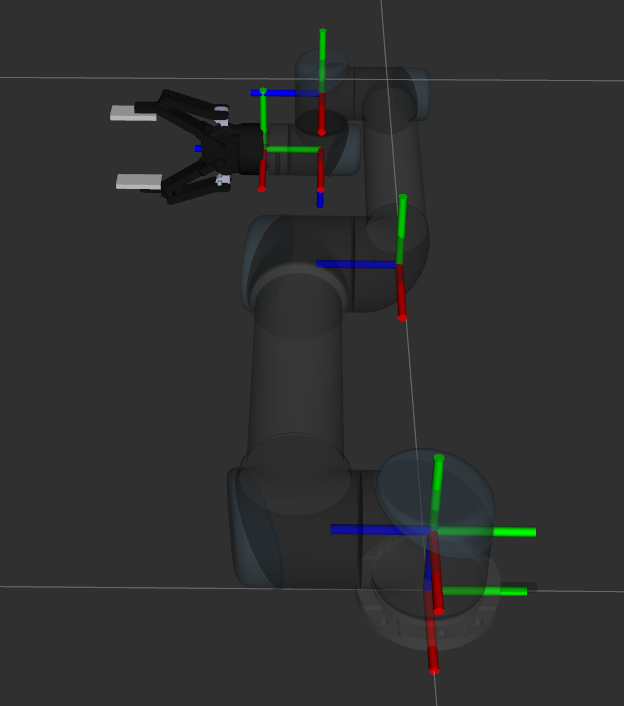
\includegraphics[width=0.48\textwidth]{images/dh_tf_frames.png}%
		\label{fig:frames-notacao-dh}%
	}%
	\hfill%
	\subfloat[Links com base no modelo URDF]{%
		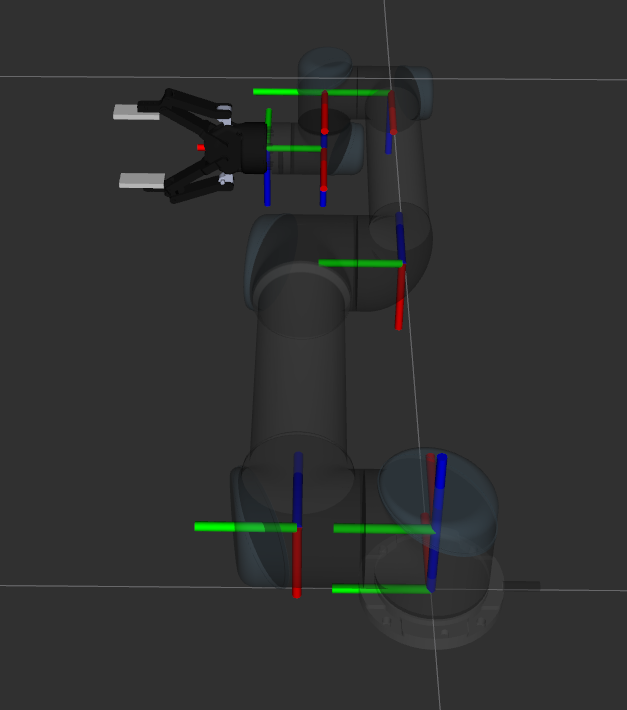
\includegraphics[width=0.48\textwidth]{images/urdf_tf_frames.png}%
		\label{fig:frames-notacao-urdf}%
	}%
\end{figure}

Após a compatibilização dos links, foi realizado a integração com a garra 2F-140 da Robotiq.
Esta integração foi realizada unindo os dois modelos através de configuração dos arquivos
URDF de ambos os modelos. Para a união foi utilizado arquivos XACRO também fornecidos
pelos respectivos fabricantes. Durante a integração ocorreram alguns problemas relacionados
a utilização da garra no Gazebo. Mais especificamente devido ao não correto funcionamento
de um \textit{plugin} e devido a um problema de renderização das \textit{meshes} dentro do simulador.
Esses problemas podem ser melhor entendidos em um 
\textit{Pull Request}\footnote{\url{https://github.com/L-eonor/robotiq/pull/1}}
realizado como solução para os pontos mencionados.

Por fim, foi criado um mundo (\textit{world}) no Gazebo formado por duas mesas, uma lata de
cerveja e o próprio manipulador UR5 já com a garra 2F-140 integrada, como está ilustrado na
Figura \ref{fig:gazebo-world}.

\begin{figure}[h]
	\centering
	\caption{Mundo criado no simulador Gazebo}
	\label{fig:gazebo-world}
	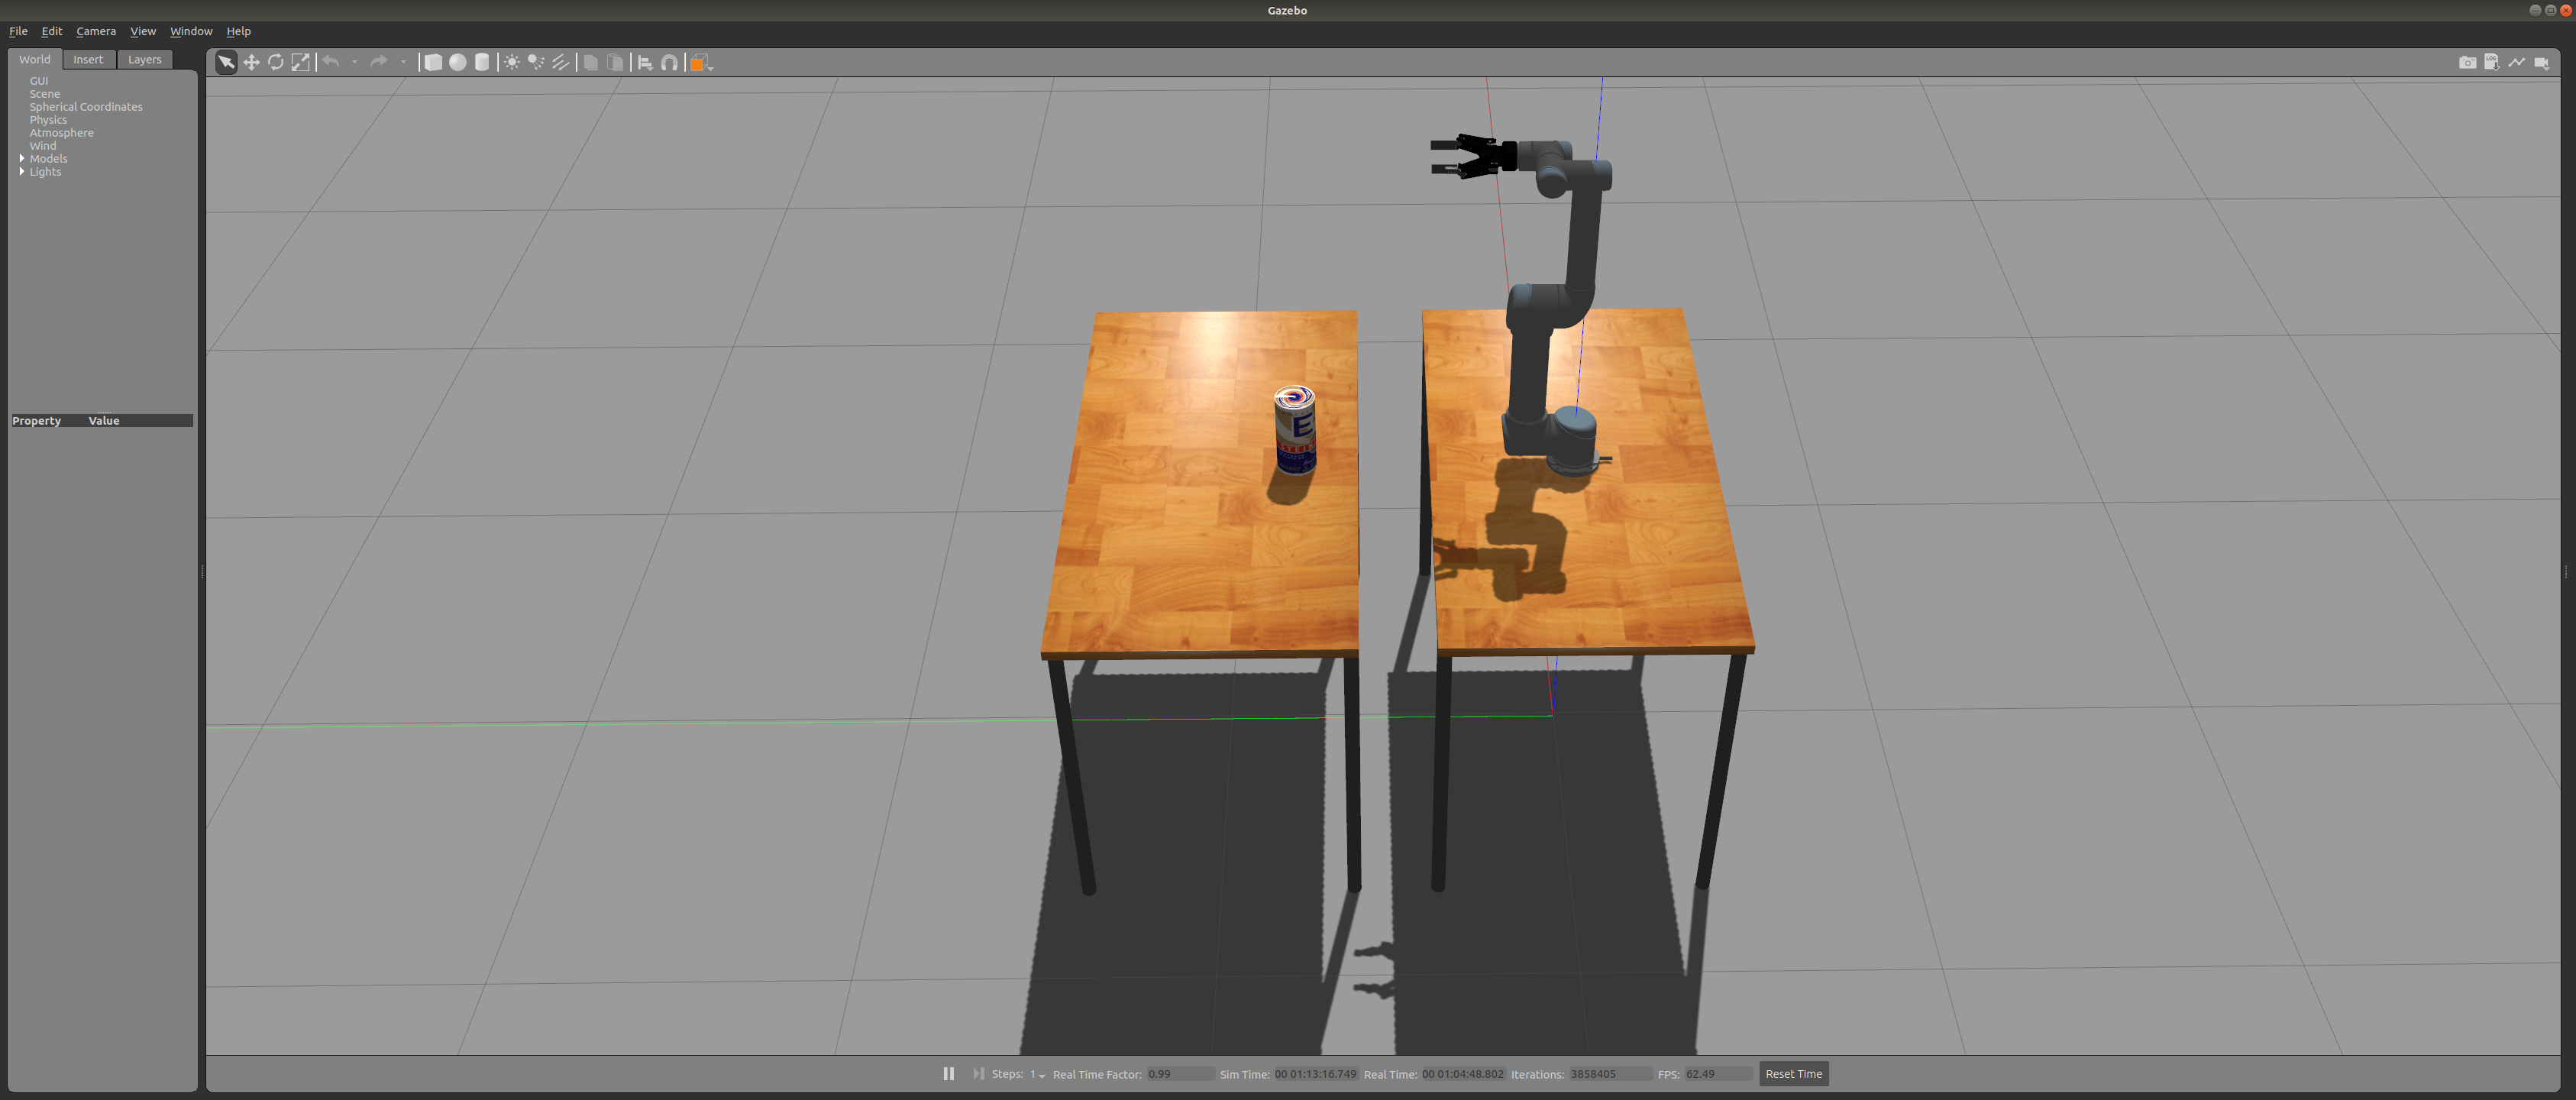
\includegraphics[width=\textwidth]{images/gazebo_world.png}
\end{figure}

O pacote criado chama-se ur5\_simulation\footnote{\url{https://github.com/mateusmenezes95/ur5_simulation}}
e encontra-se disponível para utilização da comunidade \textit{open source}. Na documentação do
pacote é explicado como utilizá-lo.

\section{Cinemática do UR5}

Os tópicos a seguir descrevem os métodos de cálculo da cinemática direta e inversa, realizados conforme \cite{Andersen2018}, 
bem como foram realizadas as validações destes cálculos usando a integração ROS/Gazebo e por fim há breve discussão dos resultados obtidos. 

\subsection{Cinemática Direta}
\label{ssec:cinematica-direta}

Para o cálculo da cinemática direta foram utilizados os parâmetros de Denavit-Hartenberg modificados,
de forma a facilitar o cálculo da transformação homogênea entre dois links consecutivos, cuja equação
é representada por \ref{eq:dh-modificado}. Os parâmetros mecânicos do UR5 utilizados para o cálculo da 
cinemática direta foram retirados do pacote ROS da Universal Robots e encontram-se na Tabela \ref{tab:tabela-dh}.

% dh parameters 
\begin{equation}\label{eq:dh-modificado}
_{i-1}^{1}\textrm{T}=\begin{bmatrix}
cos(\theta_i) & -sin(\theta_i) & 0 & \alpha _{i-1}\\ 
sin(\theta_i)cos(\alpha _{i-1})& cos(\theta_i)cos(\alpha _{i-1})  & -sin(\alpha _{i-1}) & -sin(\alpha _{i-1})d_i\\ 
sin(\theta_i)sin(\alpha _{i-1})&  cos(\theta_i)sin(\alpha _{i-1}) & cos(\alpha _{i-1}) & cos(\alpha _{i-1})d_i\\ 
0 & 0 & 0 & 1
\end{bmatrix}
\end{equation}

\begin{table}[h!]
	\centering
	\caption{Tabela de Denavit-Hartenberg modificado para o UR5}
	\label{tab:tabela-dh}
	\begin{tabular}{ c| c c c c }
		$i$ & $\alpha_{i-1}$ & $a_{i-1}$ & $d_i$ & $\theta_i$ \\ 
		\hline
		1  & 0 & 0 & $d_1 = 0.089159$ & $\theta_1$ \\  ​
		​2 & $\alpha_1=90^{\circ}$ & 0 & 0 & $\theta_2$  \\
		​3 & 0 & $a_2 = -0.42500$  & 0 & $\theta_3$ \\
		​4 & 0 & $a_3 = -0.39225$ & $d_4 = 0.10915$ & $\theta_4$ \\
		​5 & $\alpha_4=90^{\circ}$ & 0 & $d_5 = 0.09465$ & $\theta_5$ \\
		​6 & $\alpha_5=-90^{\circ}$ & 0 & $d_6 = 0.0823$ & $\theta_6$ 
	\end{tabular}
\end{table}

\subsection{Cinemática Inversa}
\label{ssec:cinematica-inversa}

No cálculo da cinemática inversa, a seguinte ordem foi seguida para obtenção dos ângulos de cada uma das juntas: $\theta_{1}$, $\theta_{5}$, $\theta_{6}$, $\theta_{3}$, $\theta_{2}$ e $\theta_{4}$. As equações para obtenção desses parâmetros estão representadas, respectivamente, em \ref{eq:theta-1}, \ref{eq:theta-5}, \ref{eq:theta-6}, \ref{eq:theta-3}, \ref{eq:theta-2} e \ref{eq:theta-4}.

% p05
\begin{equation}\label{eq:translacao-frame-5}
^{0}\textrm{P}_{5} = _{0}^{6}\textrm{T}
	\begin{bmatrix}
		0 \\ 
		0 \\ 
		-d_{6}\\ 
	\end{bmatrix}
\end{equation}

% teta1
\begin{equation}\label{eq:theta-1}
\theta _1=atan2\left (^{0}\textrm{P}_{5y}^{0}\textrm{P}_{5x}  \right )\pm acos\left ( \frac{d_4}{\sqrt{^{0}\textrm{P}_{5x}^{2}+^{0}\textrm{P}_{5y}^{2}}} \right )+\frac{\pi }{2}
\end{equation}

% teta5
\begin{equation}\label{eq:theta-5}
\theta _5=\pm acos\left ( \frac{^{0}\textrm{P}_{6x}sin(\theta _1)-^{0}\textrm{P}_{6y}cos(\theta _1)-d_4}{d_6} \right )
\end{equation}

% teta6
\begin{equation}\label{eq:theta-6}
\theta _6=atan2\left ( \frac{^{6}\textrm{X}_{0y}sin(\theta_1)+^{6}\textrm{Y}_{0y}cos(\theta_1)}{sin(\theta_5)}, \frac{^{6}\textrm{X}_{0x}sin(\theta_1)-^{6}\textrm{Y}_{0x}cos(\theta_1)}{sin(\theta_5)} \right )
\end{equation}

% teta3
\begin{equation}\label{eq:theta-3}
\theta _3 = \pm acos\left ( \frac{\left |^{1}\textrm{P}_{4xz}  \right |-a_2^2-a_3^2}{2a_2a_3} \right )
\end{equation}

% teta2
\begin{equation}\label{eq:theta-2}
\theta _2 = atan2\left (-^{1}\textrm{P}_{4z},-^{1}\textrm{P}_{4x}  \right )-asin\left ( \frac{-a_3sin(\theta3)}{\left |^{1}\textrm{P}_{4xz}  \right |} \right )
\end{equation}

% teta4
\begin{equation}\label{eq:theta-4}
\theta _4 = atan2 \left ( ^{3}\textrm{X}_{4y},^{3}\textrm{X}_{4x} \right )
\end{equation}

Note que $\theta_{1}$, $\theta_{5}$ e $\theta_{3}$ assumem dois valores possíveis. Para $\theta_{1}$,
isso corresponde ao ombro estar na posição esquerda ou direita (Figuras \ref{fig:shoulder-left} e 
\ref{fig:shoulder-right}). Para $\theta_{5}$, isso implica no pulso do robô estar na posição superior
ou inferior (Figuras \ref{fig:wrist-up} e \ref{fig:wrist-down}). Para $\theta_{3}$, os dois valores
significam a possibilidade do cotovelo estar na posição superior ou inferior (Figuras \ref{fig:elbow-up}
e \ref{fig:elbow-down}). Dadas essas possibilidades, o robô passa a ter então 8 combinações de ângulos de
juntas para alcançar determinada pose: $2\theta_{1}$ × $2\theta_{5}$ × $1\theta_{6}$ × $2\theta_{3}$ × $1\theta_{2}$ × $1\theta_{4}$.

\begin{figure}[h!]
	\centering
	\caption{Possíveis posições para as juntas $\theta_{1}$ do UR5}
	\label{fig:solucoes-inversa-shoulder}
	\subfloat[Ombro na posição esquerda]{%
		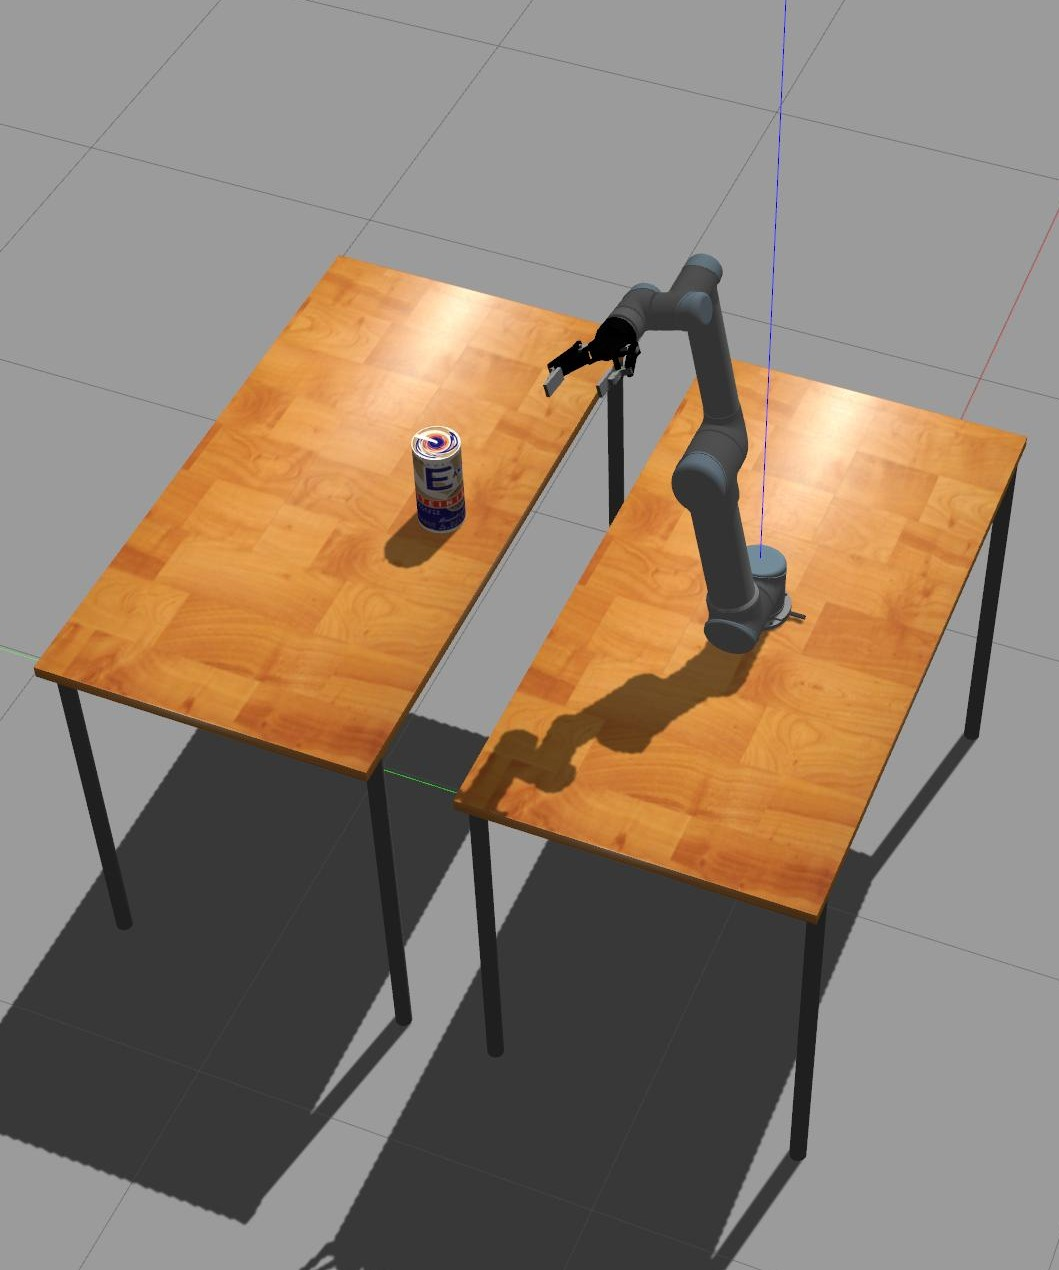
\includegraphics[width=0.4\textwidth]{images/shoulder_left.jpg}%
		\label{fig:shoulder-left}%
	}%
	\hspace{1cm}%
	\subfloat[Ombro na posição direita]{%
		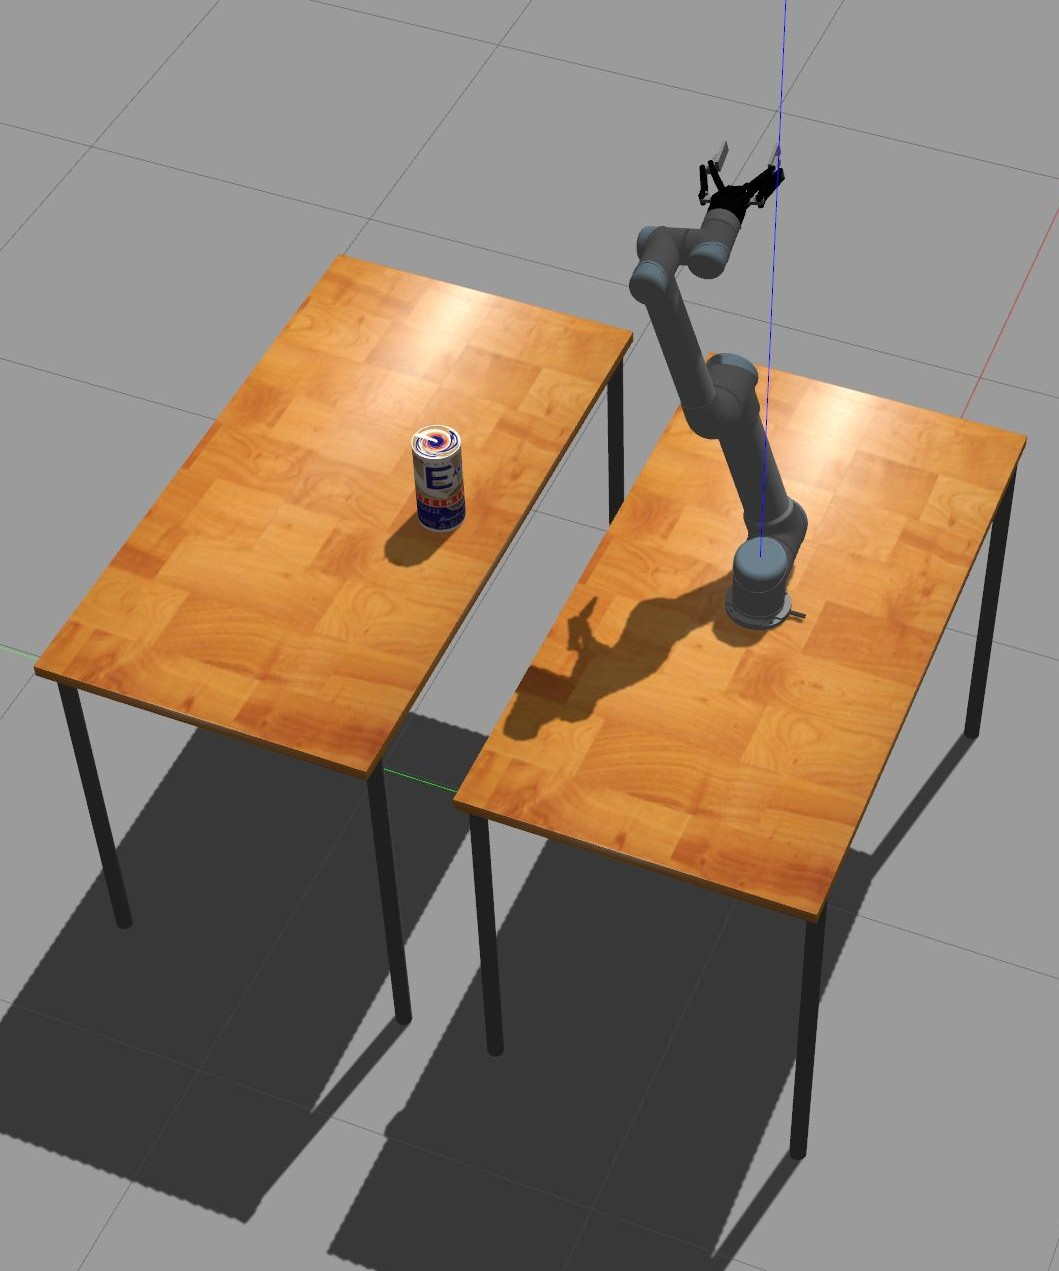
\includegraphics[width=0.4\textwidth]{images/shoulder_right.jpg}%
		\label{fig:shoulder-right}%
	}%
\end{figure}

\begin{figure}[h!]
	\centering
	\caption{Possíveis posições para as juntas $\theta_{5}$do UR5}
	\label{fig:solucoes-inversa-wrist}
	\hspace{1cm}%
	\subfloat[Pulso na posição superior]{%
		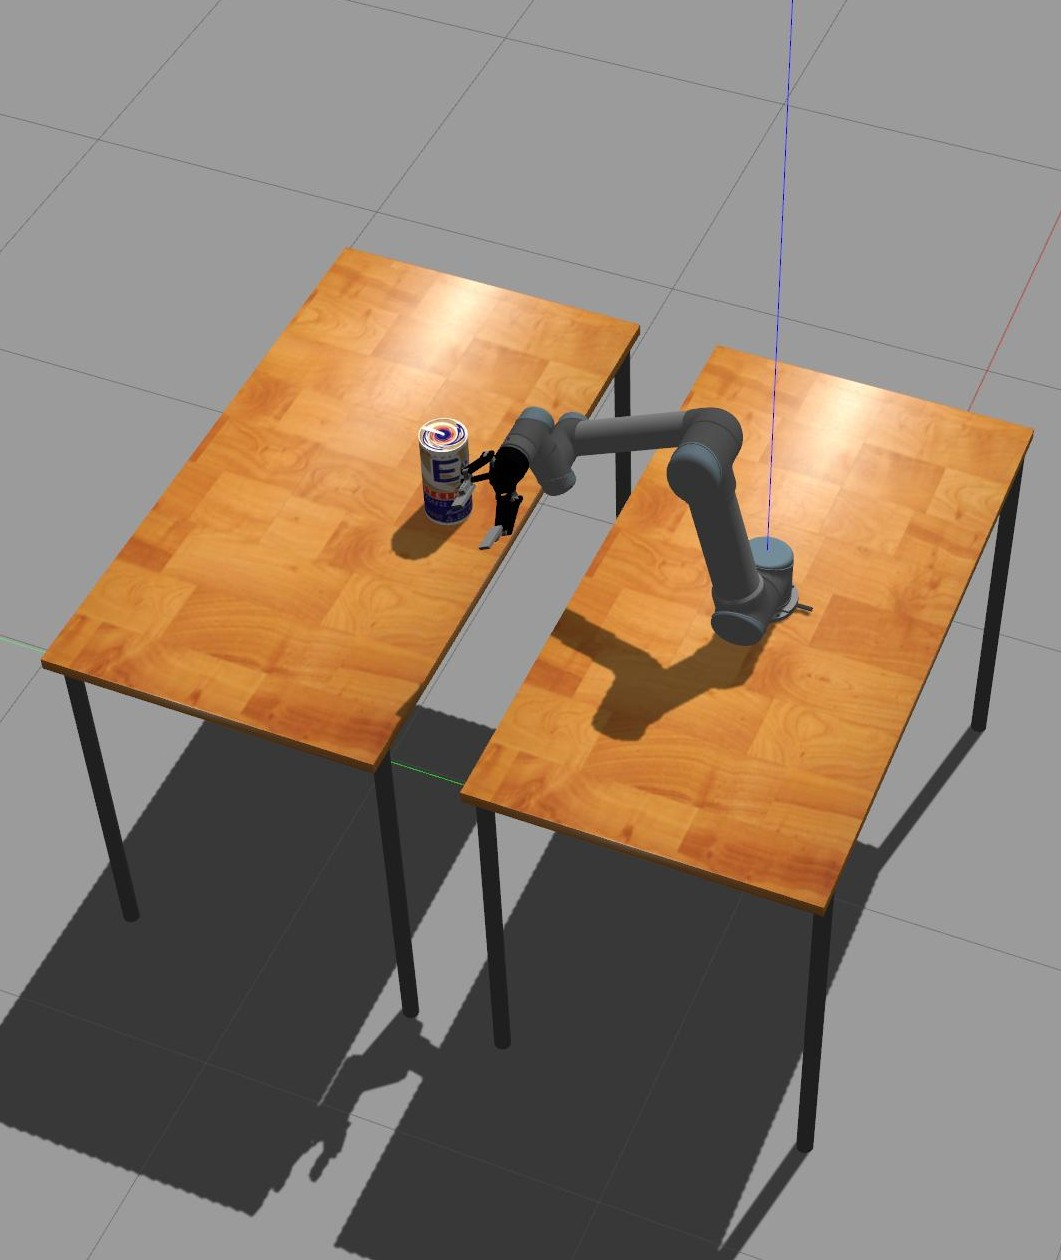
\includegraphics[width=0.4\textwidth]{images/wrist_up.jpg}%
		\label{fig:wrist-up}%
	}%
	\hspace{1cm}%
	\subfloat[Pulso na posição inferior]{%
		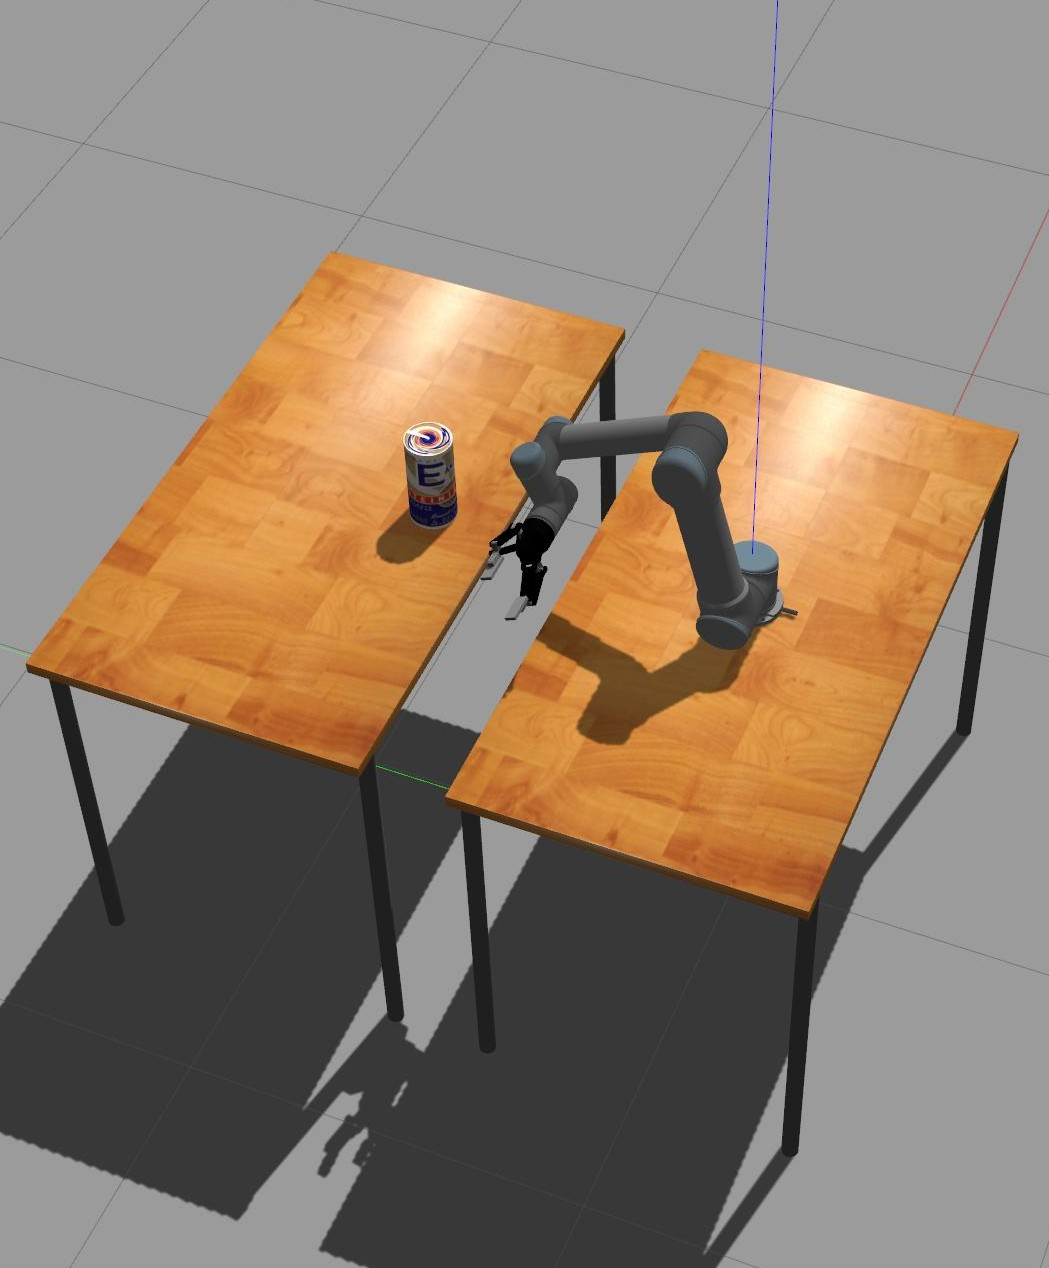
\includegraphics[width=0.4\textwidth]{images/wrist_down.jpg}%
		\label{fig:wrist-down}%
	}%
\end{figure}

\begin{figure}[h!]
	\centering
	\caption{Possíveis posições para as juntas $\theta_{3}$ do UR5}
	\label{fig:solucoes-inversa-elbow}
	\subfloat[Cotovelo na posição superior]{%
		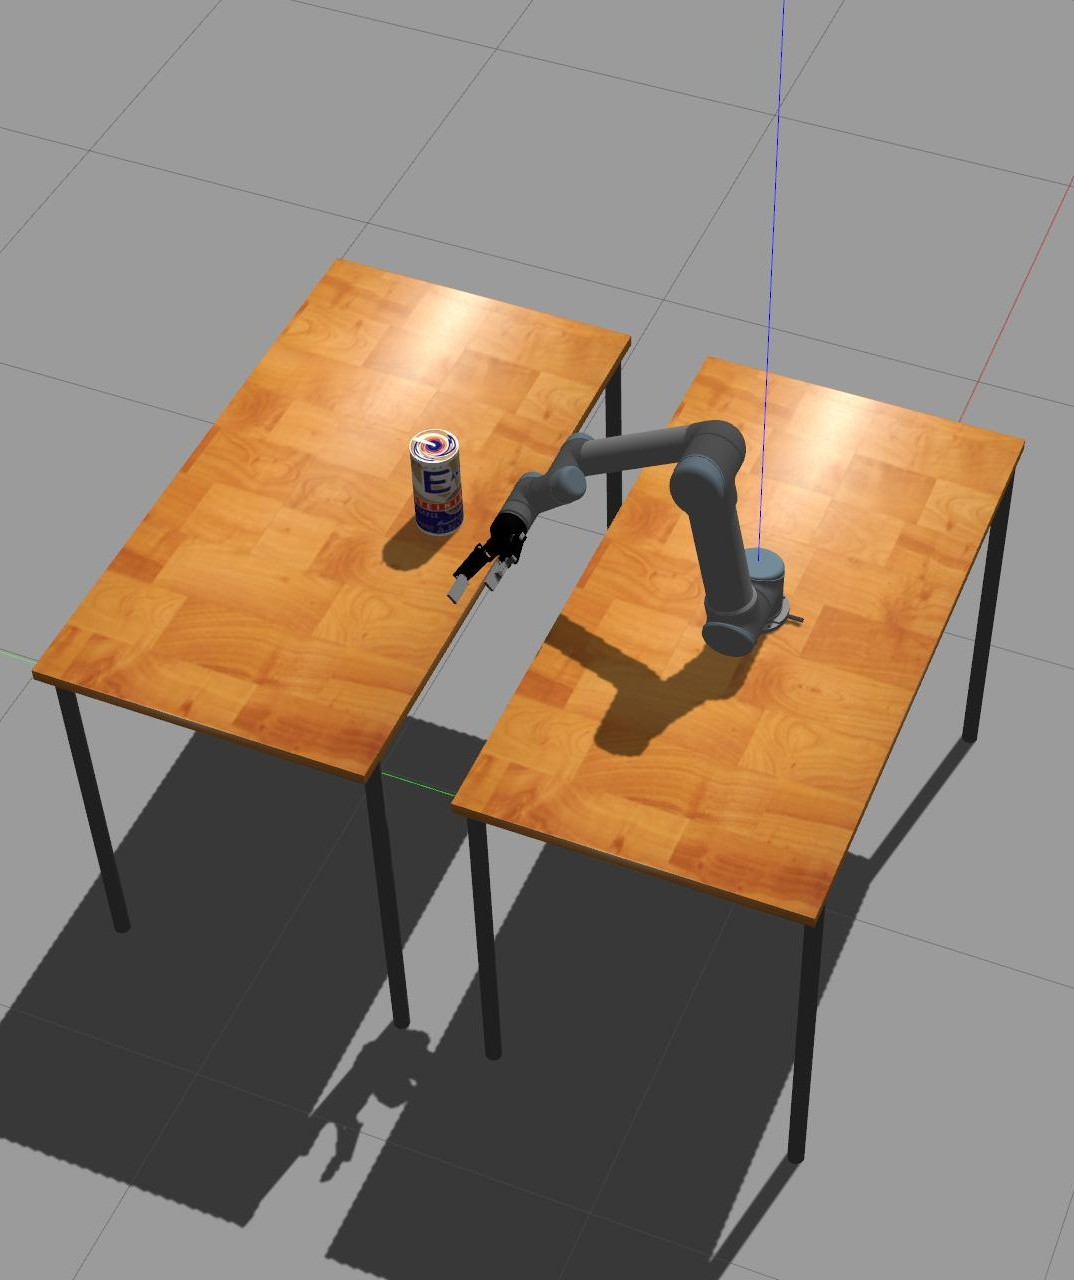
\includegraphics[width=0.39\textwidth]{images/elbow_up.jpg}%
		\label{fig:elbow-up}%
	}%
	\hspace{1cm}%
	\subfloat[Cotovelo na posição inferior]{%
		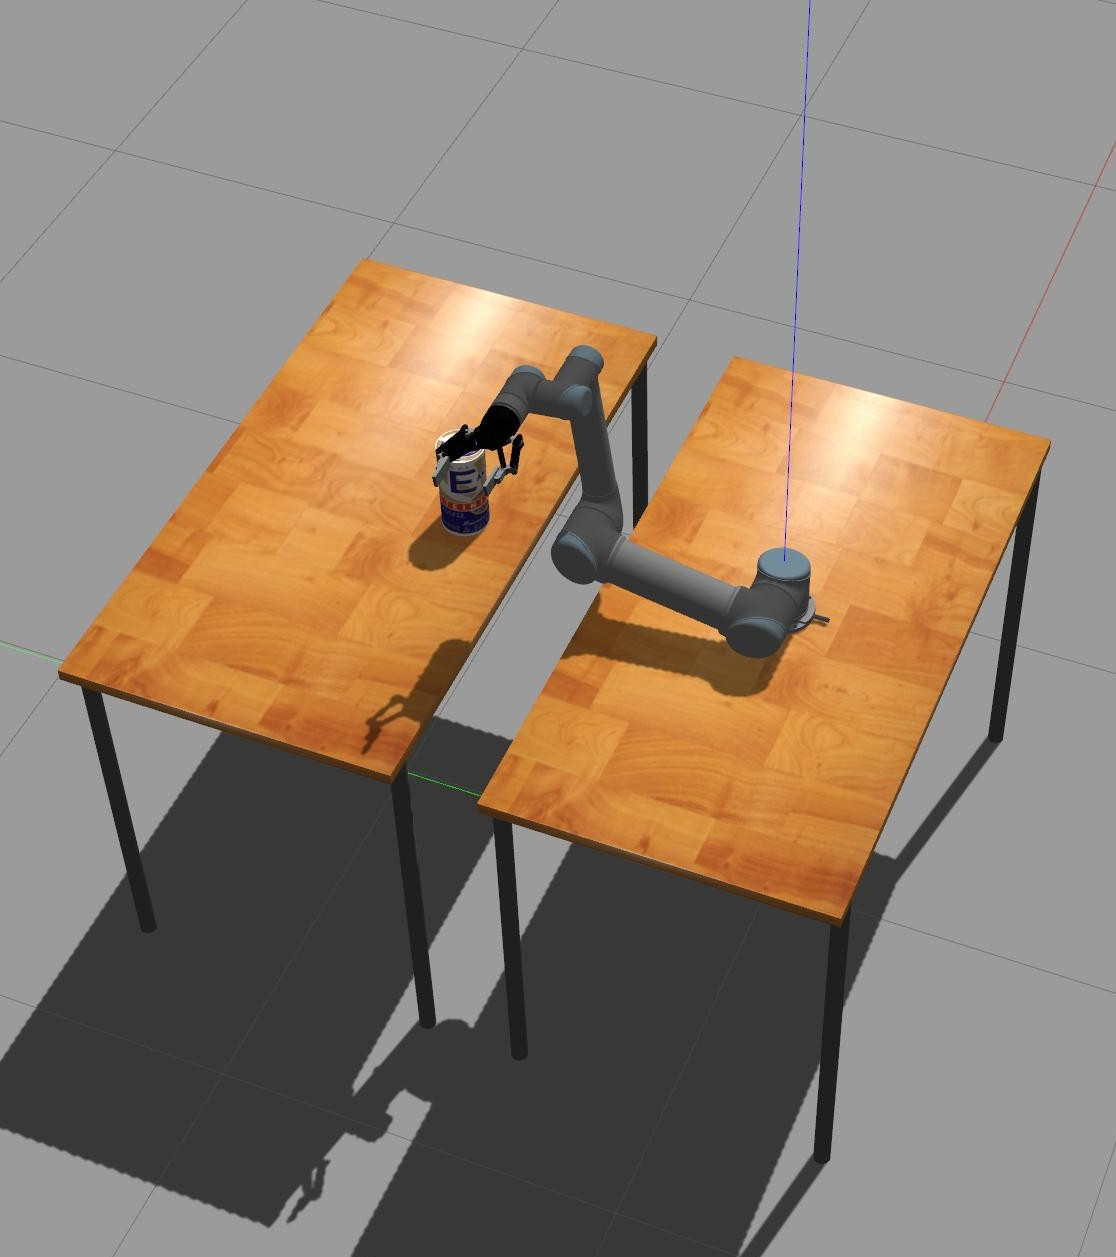
\includegraphics[width=0.42\textwidth]{images/elbow_down.jpg}%
		\label{fig:elbow-down}%
	}%
\end{figure}


\FloatBarrier
\subsection{Validação}
Para validar os métodos que calculam a cinemática direta e inversa do UR5, foram escolhidas
4 posições e orientações do \textit{end effector} do manipulador. As 4 \textit{poses} especificadas
simulam 4 posicionamentos possíveis para a garra pegar a lata que se encontra na mesa à frente
do manipulador, como pode ser visto nas Figuras \ref{fig:posicionamentos-da-garra-esq-dir} e 
\ref{fig:posicionamentos-da-garra-sup-inf}. Além disso,
foram adicionadas \textit{poses} intermediárias que antecedem o movimento final da garra
(\textit{grasp}) e a volta do robô para a \textit{pose} de \textit{home}. Estas \textit{poses}
intermediárias foram escolhidas para evitar colisões dos componentes mecânicos do manipulador,
principalmente do \textit{end effector}, com a lata de cerveja e/ou com as mesas.


\begin{figure}[htp!]
	\centering
	\caption{Posicionamentos da garra para pegar a lata pela esquerda ou direita}
	\label{fig:posicionamentos-da-garra-esq-dir}
	\subfloat[\textit{Grasp} pelo lado esquerdo]{%
		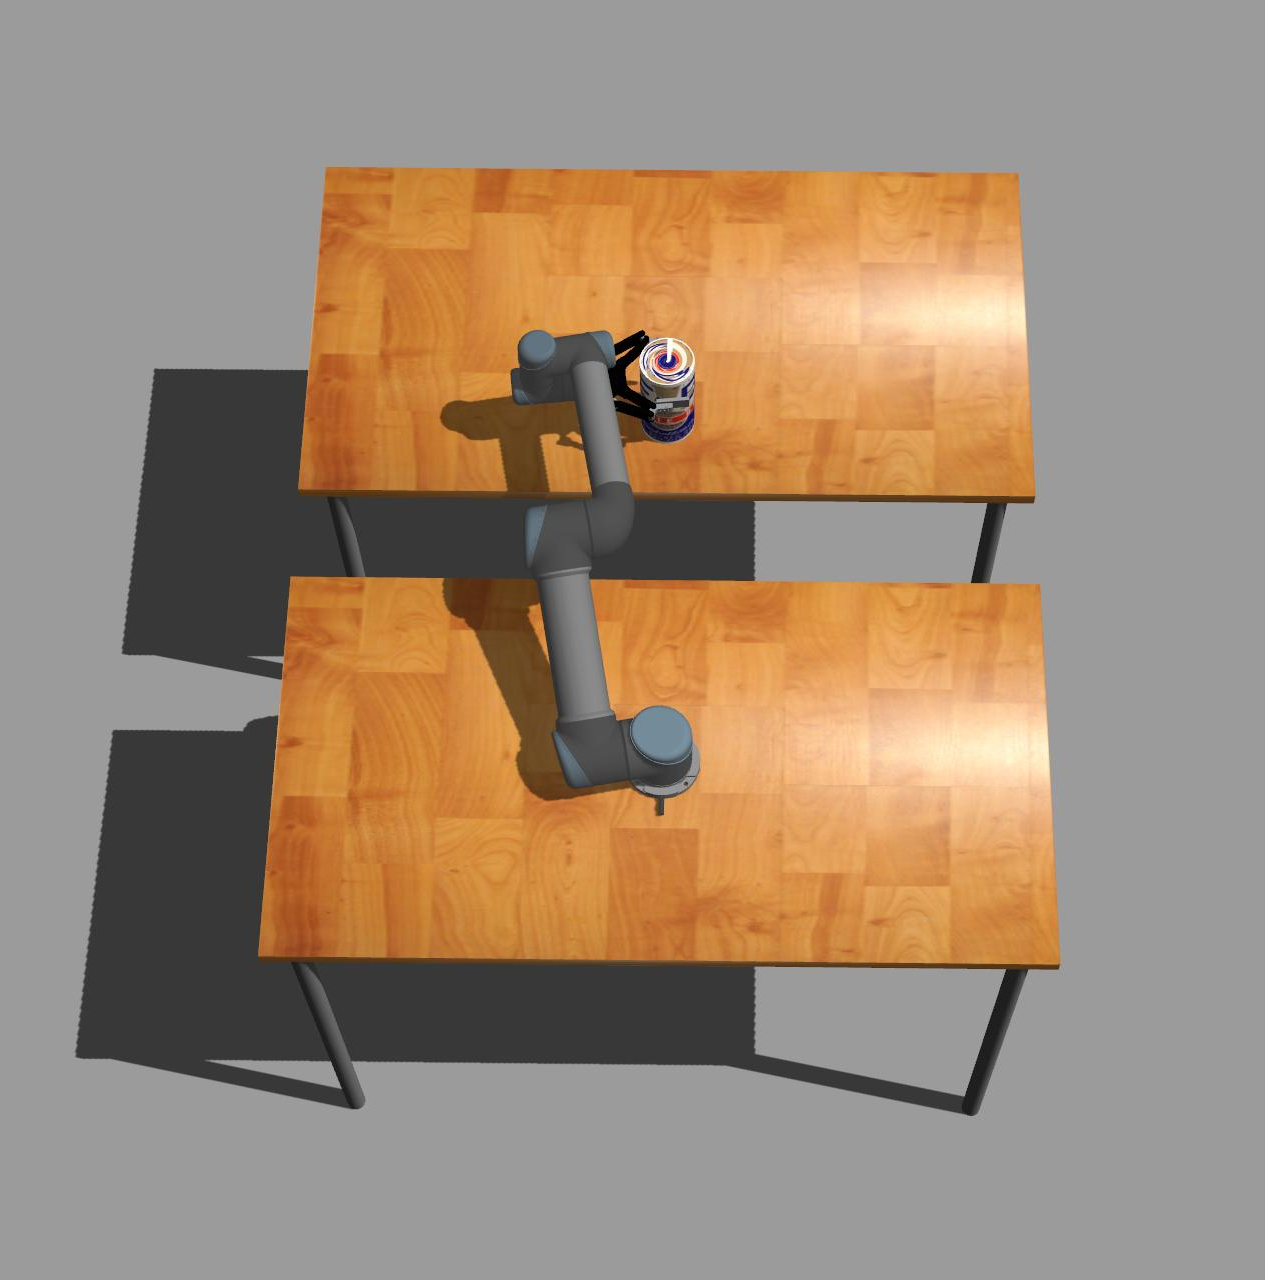
\includegraphics[width=0.45\textwidth]{images/grasp_lateral_esquerda.jpg}%
		\label{fig:grasp-lado-esquerdo}%
	}%
	\hspace{1cm}%
	\subfloat[\textit{Grasp} pelo lado direito]{%
		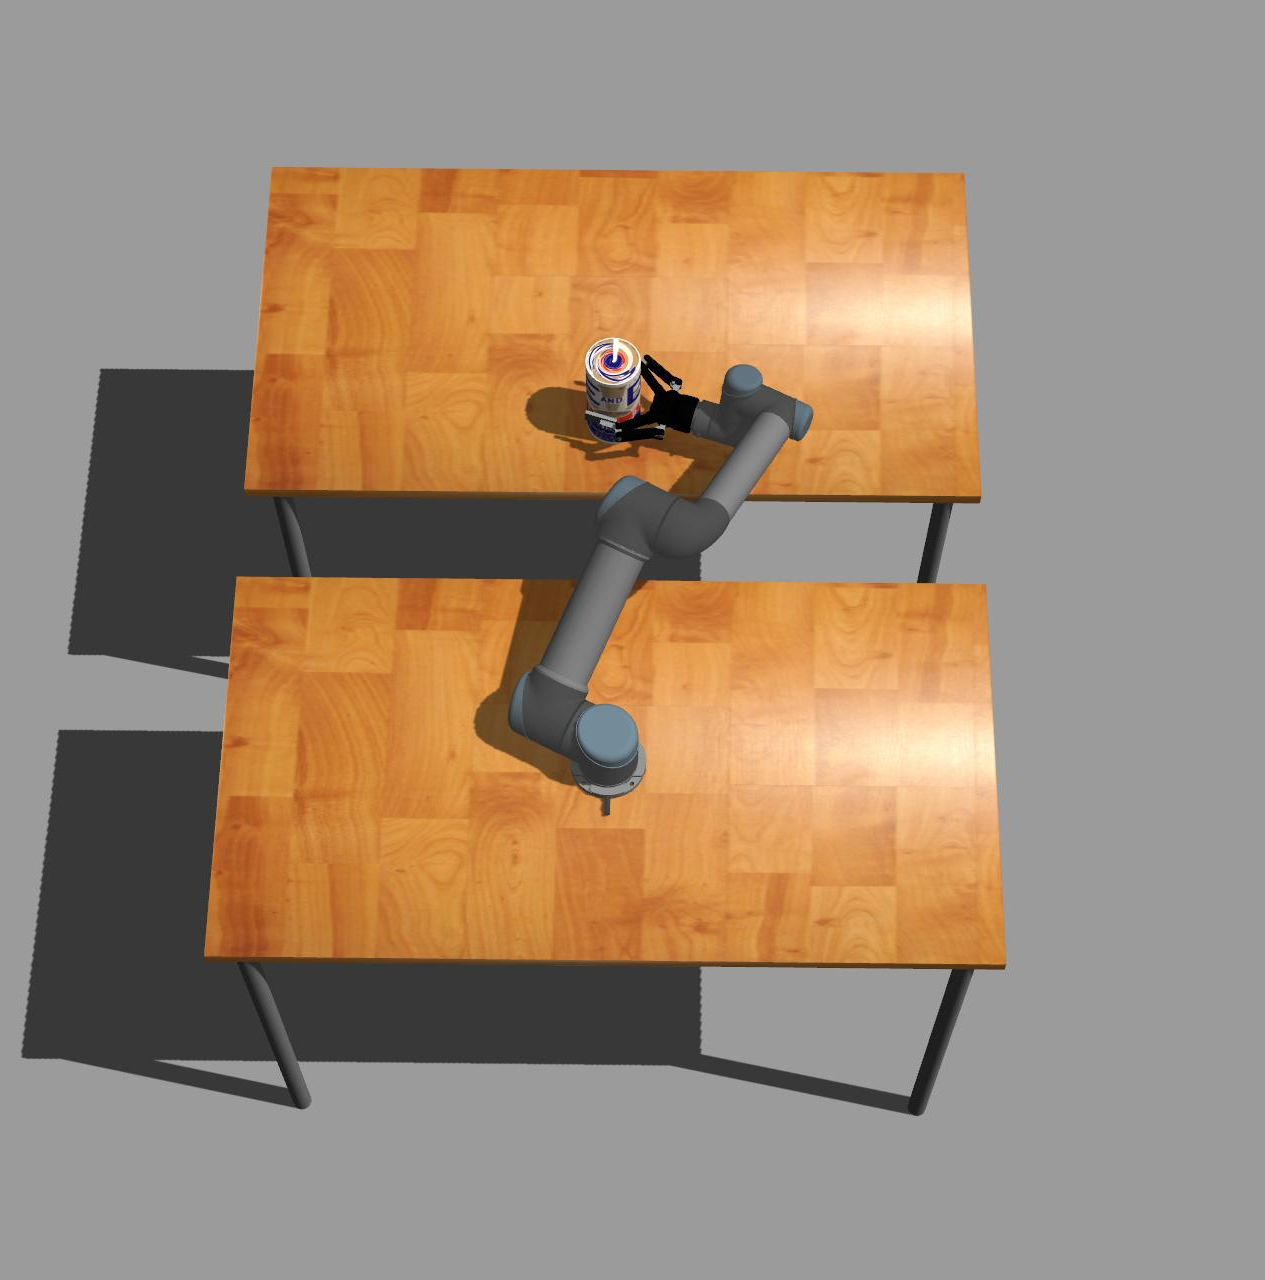
\includegraphics[width=0.45\textwidth]{images/grasp_lateral_direita.jpg}%
		\label{fig:grasp-lado-direiro}%
	}%
\end{figure}

\begin{figure}[h!]
	\centering
	\caption{Posicionamentos da garra para pegar a lata pela frente ou por cima}
	\label{fig:posicionamentos-da-garra-sup-inf}
	\subfloat[\textit{Grasp} pela frente]{%
		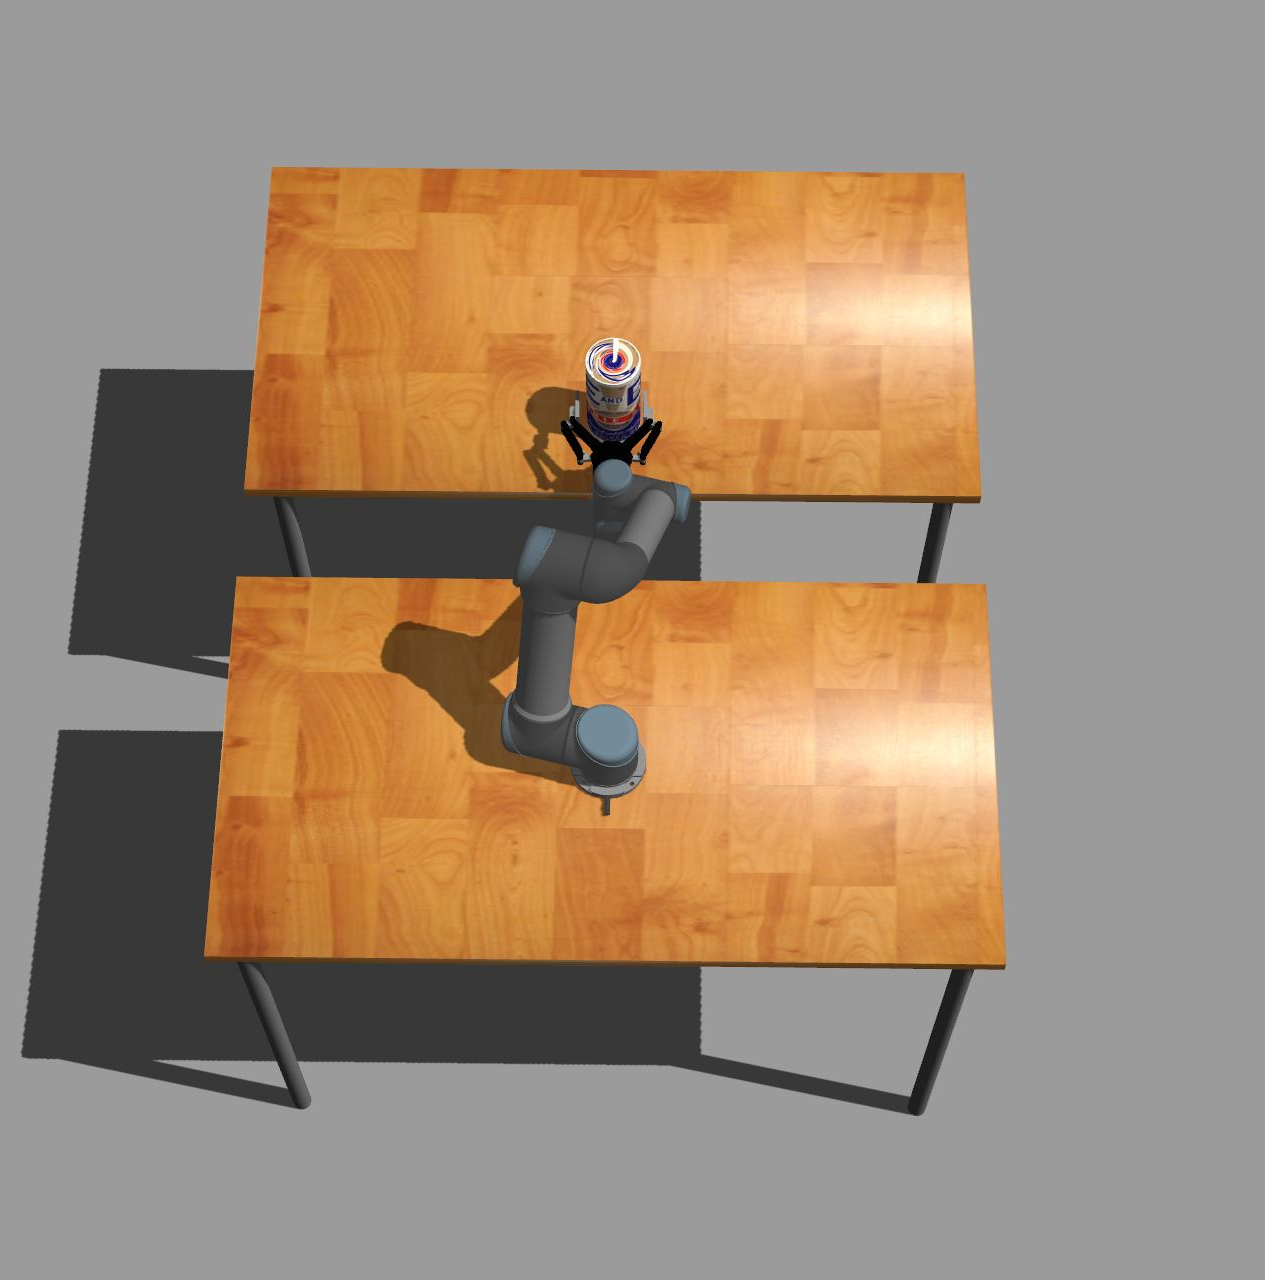
\includegraphics[width=0.45\textwidth]{images/grasp_frente.jpg}%
		\label{fig:grasp-pela-frente}%
	}%
	\hspace{1cm}%
	\subfloat[\textit{Grasp} pela parte superior]{%
		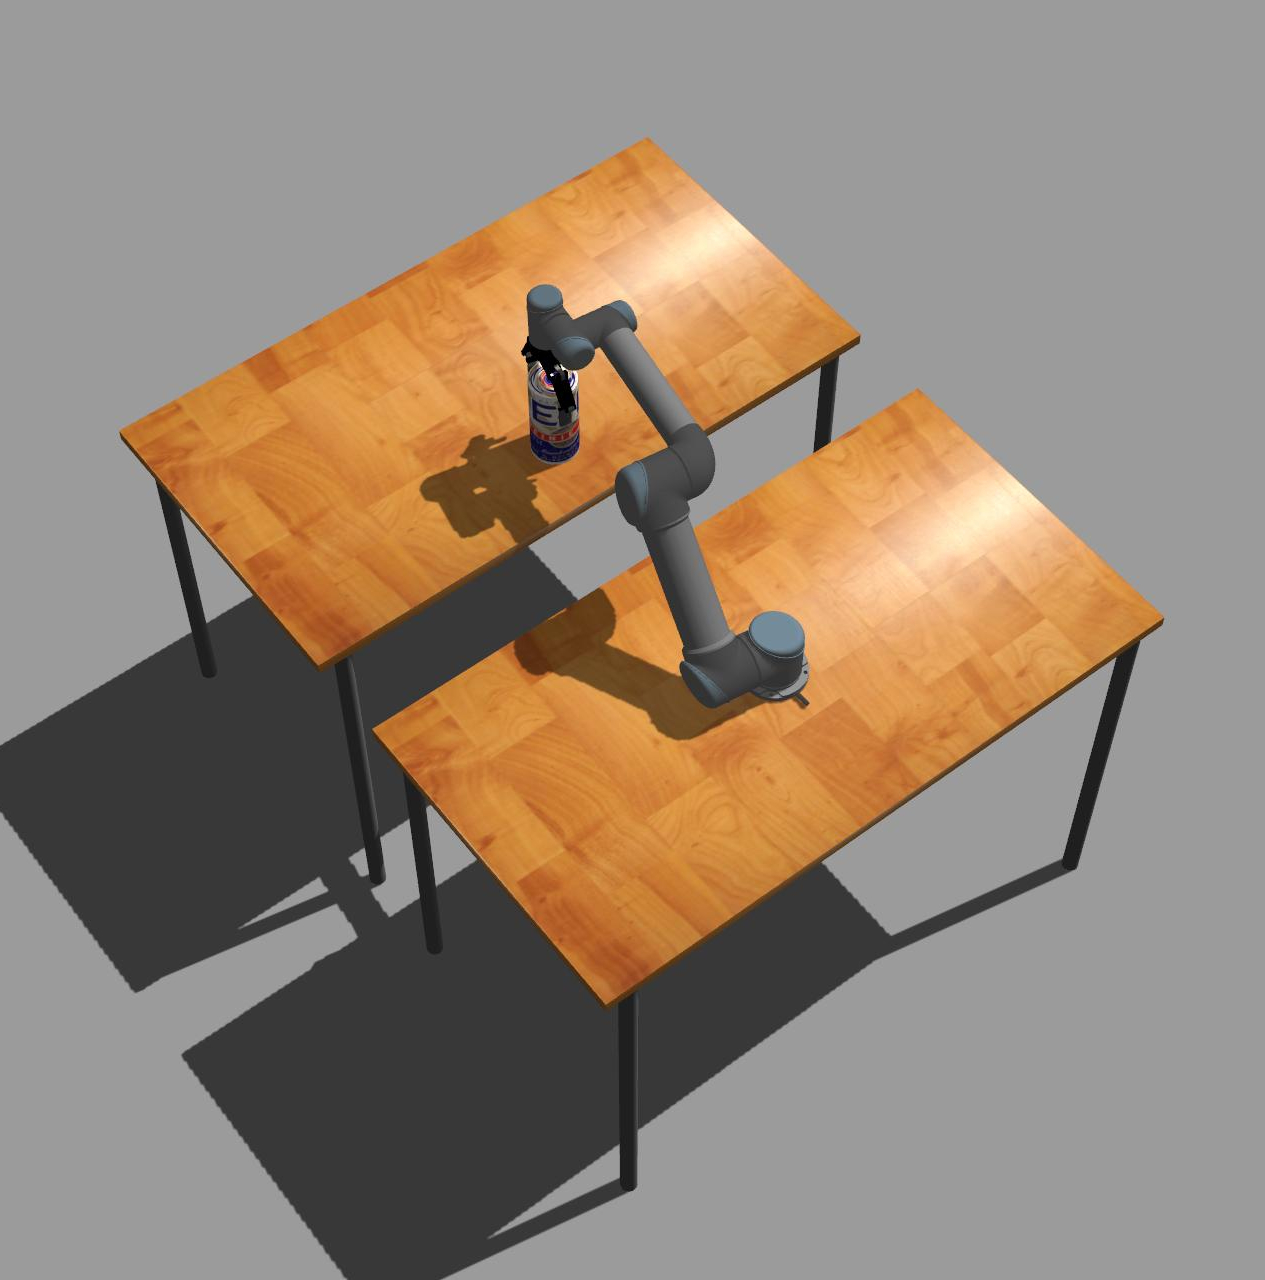
\includegraphics[width=0.45\textwidth]{images/grasp_superior.jpg}%
		\label{fig:grasp-pela-superior}%
	}%
\end{figure}

\FloatBarrier

Na Tabela \ref{tab:conjuntos-de-valores-de-juntas} estão listados os valores de juntas usados na validação do cálculo de cinemática.
As linhas foram preenchidas em cores para informar se uma determinada linha representa a \textit{pose}
de \textit{grasping}, \textit{pre/post grasping} ou \textit{home}.

\begin{table}
	\definecolor{home-gray}{gray}{0.95}
	\definecolor{pre-post-grasping-gray}{gray}{0.75}
	\definecolor{grasping-gray}{gray}{0.55}
	\centering
	\caption{Conjuntos dos valores de juntas utilizados para validação do cálculos de cinemática direta e
		inversa do UR5
	}
	\label{tab:conjuntos-de-valores-de-juntas}
	\begin{tabular}{c|c|c|c|c|c|c}
		\hline
		\rowcolor{white} 					$i$ & $\theta_{1} $ & $\theta_{2}$ & $\theta_{3}$ & $\theta_{4}$ & $\theta_{5}$ & $\theta_{6}$ \\ 
		\hline 
		\rowcolor{home-gray} 				0   &    0.00       &     -1.57    &     0.00     &     0.00     &     0.00     &     0.00     \\ 
		\hline                 
		\rowcolor{pre-post-grasping-gray} 	1   &    0.95       &     -0.47    &     0.73     &     0.00     &    -0.31     &     1.32     \\ 
		\hline                 
		\rowcolor{grasping-gray} 			2   &    1.09       &     -0.47    &     0.73     &     0.00     &    -0.20     &     1.32     \\ 
		\hline                 
		\rowcolor{pre-post-grasping-gray} 	3   &    0.95       &     -0.47    &     0.73     &     0.00     &    -0.31     &     1.32     \\ 
		\hline                 
		\rowcolor{home-gray} 				4   &    0.00       &     -1.57    &     0.00     &     0.00     &     0.00     &     0.00     \\ 
		\hline                 
		\rowcolor{pre-post-grasping-gray} 	5   &    1.94       &     -0.45    &     0.00     &     0.00     &     3.27     &     1.57     \\ 
		\hline                 
		\rowcolor{pre-post-grasping-gray} 	6   &    1.94       &     -0.45    &     0.45     &     0.00     &     3.27     &     1.57     \\ 
		\hline                 
		\rowcolor{grasping-gray} 			7   &    1.76       &     -0.45    &     0.45     &     0.00     &     3.22     &     1.57     \\ 
		\hline                 
		\rowcolor{pre-post-grasping-gray} 	8   &    1.94       &     -0.45    &     0.45     &     0.00     &     3.27     &     1.57     \\ 
		\hline                 
		\rowcolor{pre-post-grasping-gray} 	9   &    1.94       &     -0.45    &     0.00     &     0.00     &     3.27     &     1.57     \\ 
		\hline 
		\rowcolor{home-gray} 				10  &    0.00       &     -1.57    &     0.00     &     0.00     &     0.00     &     0.00     \\ 
		\hline 
		\rowcolor{pre-post-grasping-gray} 	11  &    1.00       &     -1.25    &     2.07     &     -0.75    &     1.33     &     1.57     \\ 
		\hline 
		\rowcolor{pre-post-grasping-gray} 	12  &    1.33       &     -1.25    &     2.07     &     -0.75    &     1.33     &     0.00     \\ 
		\hline 
		\rowcolor{grasping-gray} 		    13  &    1.33       &     -1.20    &     1.88     &     -0.60    &     1.31     &     1.57     \\ 
		\hline 
		\rowcolor{pre-post-grasping-gray} 	14  &    1.33       &     -1.25    &     2.07     &     -0.75    &     1.33     &     0.00     \\ 
		\hline
		\rowcolor{pre-post-grasping-gray} 	15  &    1.00       &     -1.25    &     2.07     &     -0.75    &     1.33     &     1.57     \\ 
		\hline
		\rowcolor{home-gray} 				16  &    0.00       &     -1.57    &     0.00     &     0.00     &     0.00     &     0.00     \\ 
		\hline
		\rowcolor{pre-post-grasping-gray} 	17  &    1.44       &     -0.96    &     0.75     &     -1.49    &     -1.57    &     0.00     \\ 
		\hline
		\rowcolor{grasping-gray} 			18  &    1.44       &     -0.84    &     0.75     &     -1.46    &     -1.57    &     0.00     \\ 
		\hline
		\rowcolor{pre-post-grasping-gray} 	19  &    1.44       &     -0.96    &     0.75     &     -1.49    &     -1.57    &     0.00     \\ 
		\hline
		\rowcolor{home-gray} 				20  &    0.00       &     -1.57    &     0.00     &      0.00    &      0.00    &     0.00     \\ 
		\hline
	\end{tabular}
	\\
	\begin{tabular}{cccccc}
		\textcolor{home-gray}{$\blacksquare$} & \textit{home} &
		\textcolor{pre-post-grasping-gray}{$\blacksquare$} & \textit{pre-post grasping} &
		\textcolor{grasping-gray}{$\blacksquare$} & \textit{grasping} \\
	\end{tabular}
\end{table}

\FloatBarrier

Para tornar este cálculo automático, foi criado uma rotina de programação
\footnote{\url{https://github.com/mateusmenezes95/ur5_simulation/blob/main/scripts/joints_controller_node.py}}
usando a linguagem Python, e APIs 
(\textit{Application Programming Interface}) e ferramentas fornecidas pelo \textit{framework}
ROS. Os conjuntos de valores de juntas listados na Tabela \ref{tab:conjuntos-de-valores-de-juntas} foram inseridos em um arquivo
de configuração\footnote{\url{https://github.com/mateusmenezes95/ur5_simulation/blob/main/config/arm_kinematics.yaml}} 
com formato YAML (acrônimo recursivo para \textit{YAML Ain't Markup Language}).
Então para cada conjunto de valores de juntas lidos do arquivo de configuração, foi feito
a comparação entre os valores calculados pelos métodos criados e os valores fornecidos pelo 
ambiente de simulação que foram obtidos por intermédio do \textit{framework} ROS.
Ao final da rotina são gerados gráficos cujo objetivo é ter uma interpretação gráfica dos erros
obtidos entre as duas formas de aquisição dos valores da cinemática direta e inversa do UR5.
A Figura \ref{fig:fluxograma-rotina} ilustra o fluxo desta rotina.

\begin{figure}[htp]
	\centering
	\caption{Fluxograma da validação do cálculo de cinemática direta e inversa do UR5}
	\label{fig:fluxograma-rotina}
	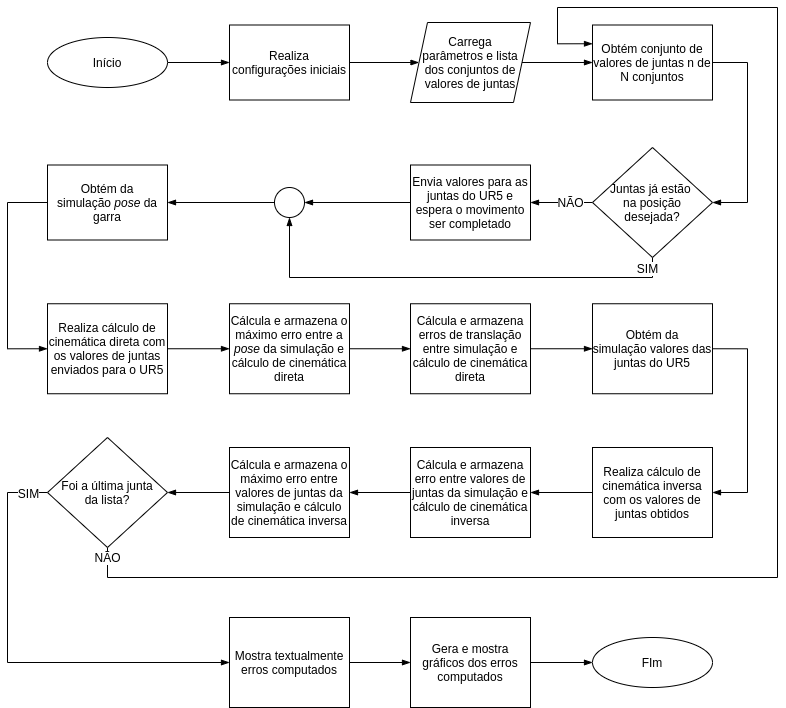
\includegraphics[width=\textwidth]{images/fluxograma_da_validacao_do_calculo_de_cinematica_direta_e_inversa.png}
\end{figure} 

\FloatBarrier

Para o conjunto de juntas da Tabela \ref{tab:conjuntos-de-valores-de-juntas}, foram gerados os gráficos de comparação
ilustrados nas Figuras \ref{fig:grafico-erro-juntas}, \ref{fig:grafico-erro-transalacao} e
\ref{fig:grafico-maximo-erros}. O cálculo do erro máximo e de translação para cinemática direta
foram realizados conforme as Equações \ref{eq:erro-max-cinematica-direta} e \ref{eq:erro-de-translacao},
respectivamente. Já as Equações \ref{eq:erro-de-valores-de-juntas} e \ref{eq:max-erro-de-valores-de-juntas}
mostram, respectivamente, como foi computado o erro dos valores de juntas e erro máximo nos
cálculos da cinemática inversa do UR5. Como métrica para o cálculo do erro entre os valores 
previstos de ângulos das juntas e os  calculados pela cinemática inversa, foi utilizado a função cosseno,
uma vez que, ângulos defasados entre si de 2$\pi$ – o que foi notado no cálculo de $\theta_{5}$ – irão sempre
apresentar o mesmo valor de cosseno.

\begin{equation}\label{eq:erro-max-cinematica-direta}
	\begin{split}
		max\_erro = &\: max \left (\left | T_s{_{0}^{6}}\right | - \left | T_c{_{0}^{6}}\right | \right) \quad \quad\\
		= &\: max \left ( \left |
		\begin{bmatrix}
			r_{s_{11}} & r_{s_{12}} & r_{s_{13}} & o_{s_{x}} \\ 
			r_{s_{21}} & r_{s_{22}} & r_{s_{23}} & o_{s_{y}} \\ 
			r_{s_{31}} & r_{s_{32}} & r_{s_{33}} & o_{s_{z}} \\ 
			    0      &      0     &      0     &      1
		\end{bmatrix}
		\right |
		-
		\left |
		\begin{bmatrix}
			r_{c_{11}} & r_{c_{12}} & r_{c_{13}} & o_{c_{x}} \\ 
			r_{c_{21}} & r_{c_{22}} & r_{c_{23}} & o_{c_{y}} \\ 
			r_{c_{31}} & r_{c_{32}} & r_{c_{33}} & o_{c_{z}} \\ 
			    0      &      0     &      0     &      1
		\end{bmatrix}
		\right | \right )
	\end{split}
\end{equation}

\begin{equation}\label{eq:erro-de-translacao}
	\begin{split}
		o_e{_{0}^{6}} = &\: o_s{_{0}^{6}} - o_c{_{0}^{6}}\\
		= &\:
		\begin{bmatrix}
			o_{s_{x}} \\ 
			o_{s_{y}} \\ 
			o_{s_{z}}
		\end{bmatrix}
		-
		\begin{bmatrix}
			o_{c_{x}} \\ 
			o_{c_{y}} \\ 
			o_{c_{z}}
		\end{bmatrix}
	\end{split}
\end{equation}

\begin{equation}\label{eq:erro-de-valores-de-juntas}
	\begin{bmatrix}
		e_{1} \\ 
		e_{2} \\ 
		e_{3} \\
		e_{4} \\
		e_{5} \\
		e_{6}
	\end{bmatrix}
	=
	\begin{bmatrix}
		cos(\theta_{s_{1}}) \\ 
		cos(\theta_{s_{2}}) \\ 
		cos(\theta_{s_{3}}) \\
		cos(\theta_{s_{4}}) \\
		cos(\theta_{s_{5}}) \\
		cos(\theta_{s_{6}})
	\end{bmatrix}
-
	\begin{bmatrix}
		cos(\theta_{c_{1}}) \\ 
		cos(\theta_{c_{2}}) \\ 
		cos(\theta_{c_{3}}) \\
		cos(\theta_{c_{4}}) \\
		cos(\theta_{c_{5}}) \\
		cos(\theta_{c_{6}})
	\end{bmatrix}
\end{equation}

\begin{equation}\label{eq:max-erro-de-valores-de-juntas}
	 max\_\theta_{e} = max\left(\left|
	\begin{bmatrix}
		e_{1} \\ 
		e_{2} \\ 
		e_{3} \\
		e_{4} \\
		e_{5} \\
		e_{6}
	\end{bmatrix}
	\right|\right)
\end{equation}

onde os sobrescritos $s$ e $c$ representam os valores obtidos da simulação e do cálculo próprio,
respectivamente.

Observa-se na Figura \ref{fig:grafico-maximo-erros} que o maior erro absoluto obtido para o cálculo da
cinemática direta foi de 0.00167 para o conjunto 4. Observa-se que os conjuntos que mais apresentaram
erros foram os de \textit{home} números 0, 4, 10, 16 e 20. Uma hipótese para estes erros é o ruído que a
simulação fornece quando as juntas estão na posição zero e, portanto, seria embutido no cálculo de erro
um \textit{bias} com um valor milesimal.

\begin{figure}[htp]
	\centering
	\caption{Comparação dos erros máximos obtidos no cálculo de cinemática direta e inversa
		para cada conjunto $i$ de valores de juntas
	}
	\label{fig:grafico-maximo-erros}
	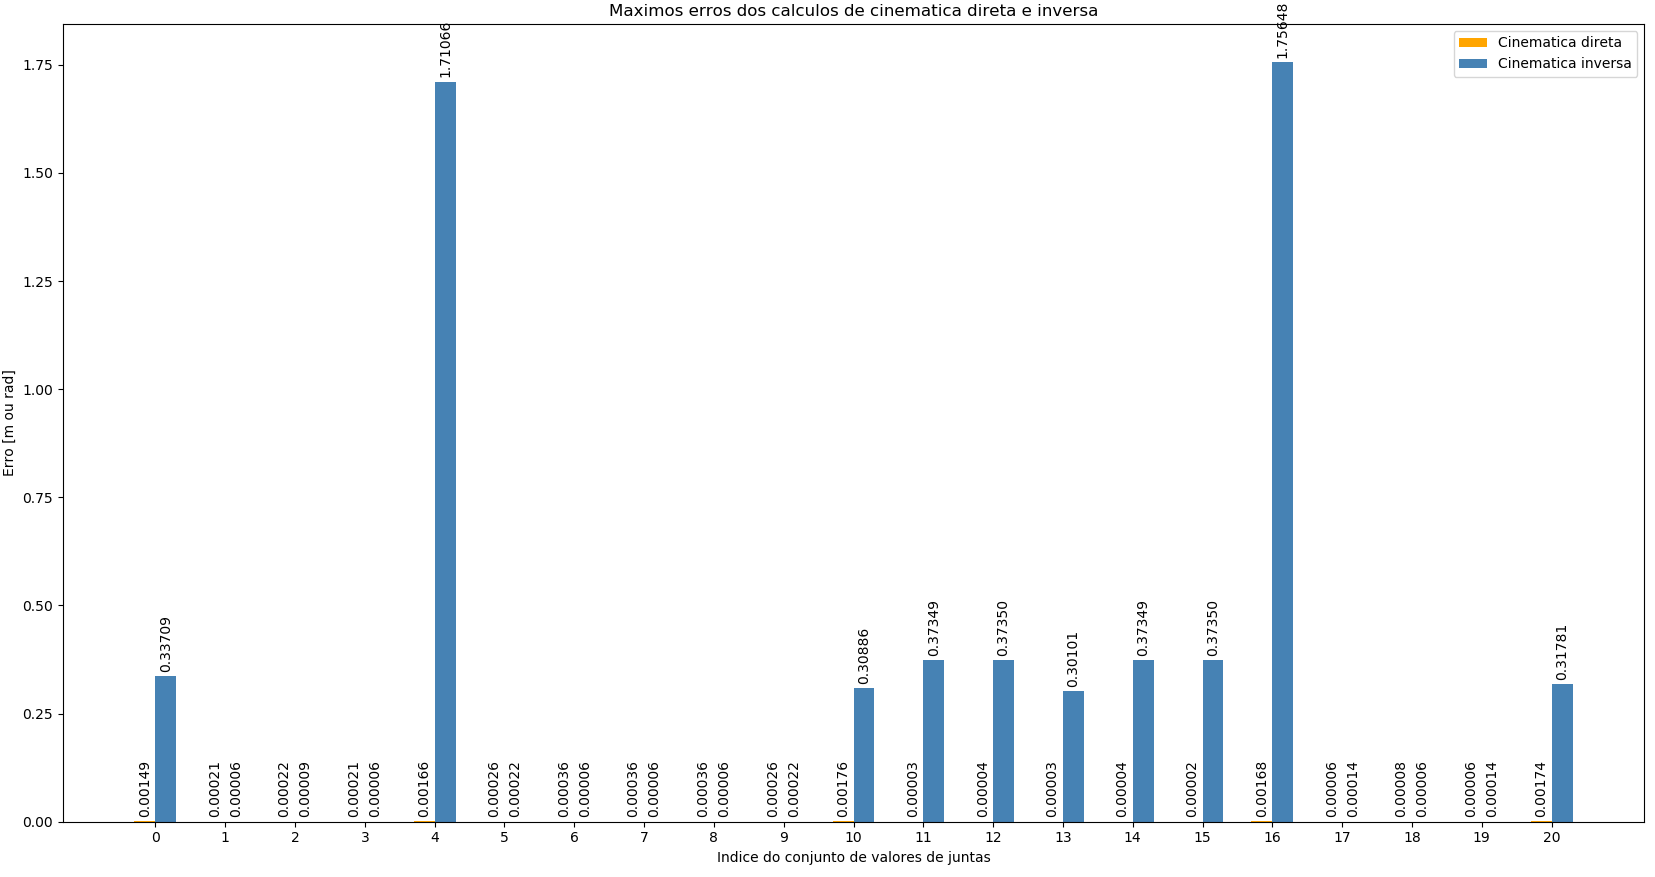
\includegraphics[width=\textwidth]{images/maximos_erros.png}
\end{figure}

O erro de translação do cálculo da Cinemática direta do UR5 pode ser visualizado na Figura \ref{fig:grafico-erro-transalacao}.
Nota-se que o erro máximo foi de aproximadamente 0,4 mm para o conjunto 4. Observa-se novamente também que os maiores erros estão nos conjuntos
de \textit{home} (0, 4, 10, 16 e 20). Entretanto, vale salientar que em uma aplicação real o erro na posição do \textit{end effector} pode ser
desconsiderado, já que nessa posição o manipulador não executa nenhuma tarefa de precisão.

\begin{figure}[htp]
	\centering
	\caption{Erros de translação da garra integrado ao UR5 para cada conjunto $i$ de valores de juntas}
	\label{fig:grafico-erro-transalacao}
	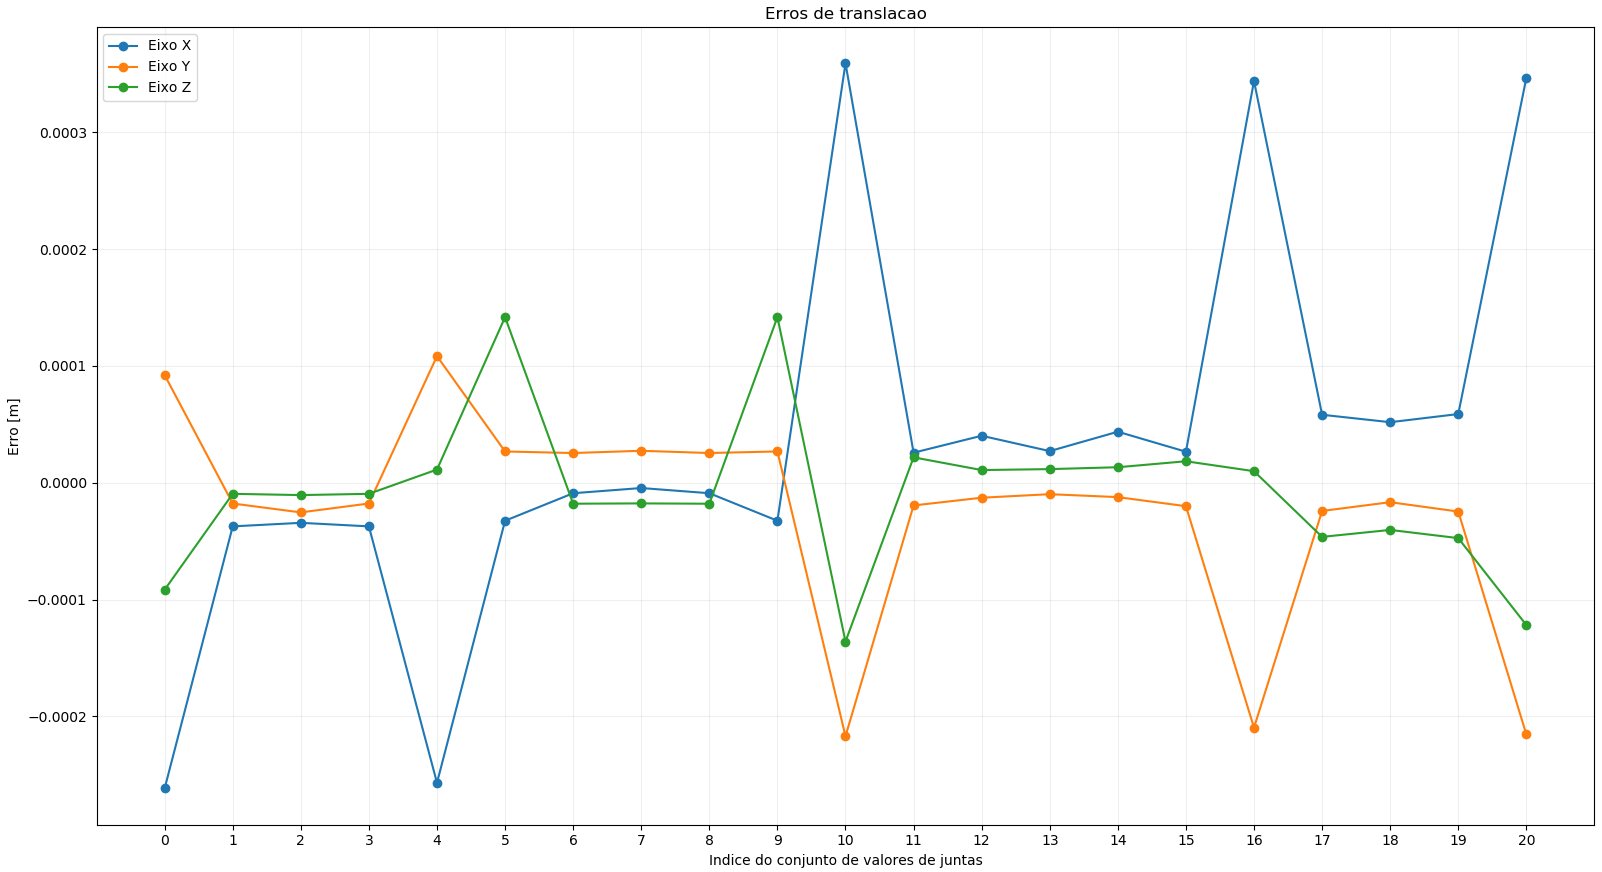
\includegraphics[width=\textwidth]{images/erros_de_translacao.png}
\end{figure}

\FloatBarrier

Na Figura \ref{fig:grafico-erro-juntas} verifica-se que do
conjunto 11 ao 15 há um erro quase que constante para a junta $\theta_{5}$, modificando apenas no conjunto
13 (conjunto de \textit{grasp} conforme Tabela \ref{tab:conjuntos-de-valores-de-juntas}). Este erro é explicado
devido principalmente a consideração da posição do UR5. Conforme explicado em \ref{ssec:cinematica-inversa} 
o valor de $\theta_{5}$ é influenciado pela posição do pulso do robô, que para o resultado da Figura \ref{fig:grafico-erro-transalacao}
foi considerada a posição superior. Fazendo um recorte da Tabela \ref{tab:conjuntos-de-valores-de-juntas}, 
gerando a nova Tabela \ref{tab:conjuntos-de-valores-de-juntas-recortado} e considerando agora o pulso na
posição inferior, obtemos os gráficos mostrados nas Figuras \ref{fig:max-erros-set-2} e \ref{fig:grafico-erro-juntas-set-2}.
Verifica-se agora que os erros se aproximam de zero para a maioria das juntas, com exceção para os conjuntos de \textit{home}.
A diferença dos resultados entre as Figuras \ref{fig:grafico-erro-juntas} e \ref{fig:grafico-erro-juntas-set-2} pode ser
explicada devido as múltiplas soluções encontradas no cálculo da cinemática inversa para o mesmo valor de junta,
conforme explicado no tópico \ref{ssec:cinematica-inversa}.

\begin{figure}[htp]
	\centering
	\caption{Erros das 6 juntas do UR5 para cada conjunto $i$ de valores de juntas}
	\label{fig:grafico-erro-juntas}
	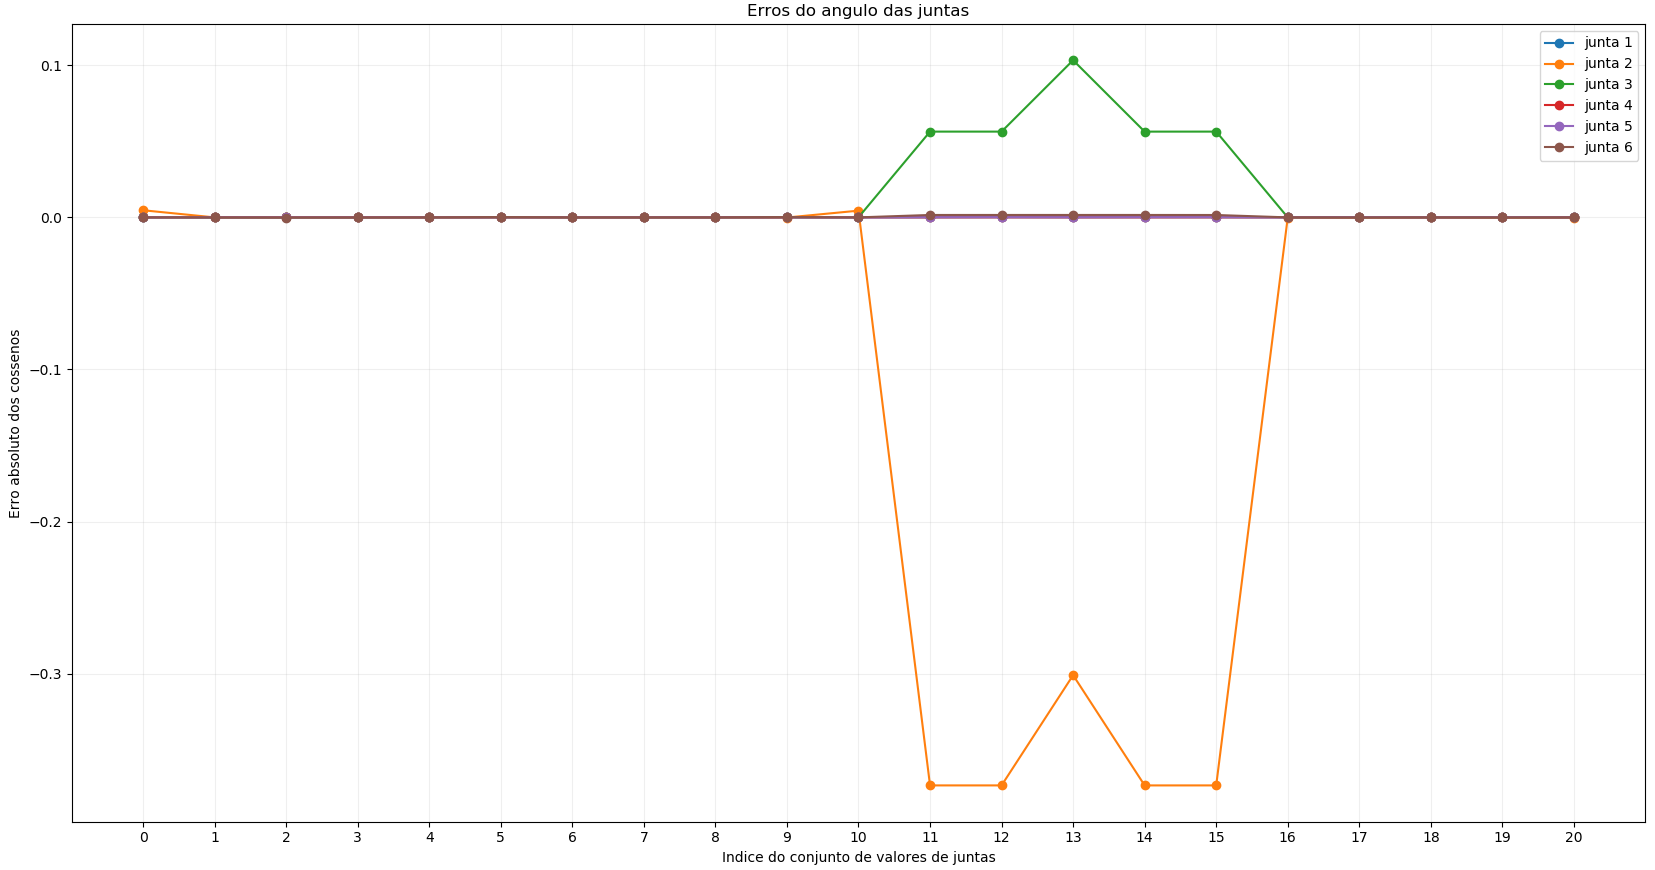
\includegraphics[width=\textwidth]{images/erro_do_angulo_das_juntas.png}
\end{figure}

\FloatBarrier

\begin{table}[htp!]
	\definecolor{home-gray}{gray}{0.95}
	\definecolor{pre-post-grasping-gray}{gray}{0.75}
	\definecolor{grasping-gray}{gray}{0.55}
	\centering
	\caption{Conjuntos dos valores de juntas recortados utilizados para validação do cálculos de cinemática direta e 
		inversa do UR5
	}
	\label{tab:conjuntos-de-valores-de-juntas-recortado}
	\begin{tabular}{c|c|c|c|c|c|c}
		\hline
		\rowcolor{white} 					$i$ & $\theta_{1} $ & $\theta_{2}$ & $\theta_{3}$ & $\theta_{4}$ & $\theta_{5}$ & $\theta_{6}$ \\ 
		\hline 
		\rowcolor{home-gray} 				0  &    0.00       &     -1.57    &     0.00     &     0.00     &     0.00     &     0.00     \\ 
		\hline 
		\rowcolor{pre-post-grasping-gray} 	1  &    1.00       &     -1.25    &     2.07     &     -0.75    &     1.33     &     1.57     \\ 
		\hline 
		\rowcolor{pre-post-grasping-gray} 	2  &    1.33       &     -1.25    &     2.07     &     -0.75    &     1.33     &     0.00     \\ 
		\hline 
		\rowcolor{grasping-gray} 		    3  &    1.33       &     -1.20    &     1.88     &     -0.60    &     1.31     &     1.57     \\ 
		\hline 
		\rowcolor{pre-post-grasping-gray} 	4  &    1.33       &     -1.25    &     2.07     &     -0.75    &     1.33     &     0.00     \\ 
		\hline
		\rowcolor{pre-post-grasping-gray} 	5  &    1.00       &     -1.25    &     2.07     &     -0.75    &     1.33     &     1.57     \\ 
		\hline
		\rowcolor{home-gray} 				6  &    0.00       &     -1.57    &     0.00     &     0.00     &     0.00     &     0.00     \\ 
		\hline
	\end{tabular}
	\\
	\begin{tabular}{cccccc}
		\textcolor{home-gray}{$\blacksquare$} & \textit{home} &
		\textcolor{pre-post-grasping-gray}{$\blacksquare$} & \textit{pre-post grasping} &
		\textcolor{grasping-gray}{$\blacksquare$} & \textit{grasping} \\
	\end{tabular}
\end{table}

\begin{figure}[htp]
	\centering
	\caption{Comparação dos erros máximos da cinemática direta e inversa
		das 6 juntas do UR5 para cada conjunto da Tabela \ref{tab:conjuntos-de-valores-de-juntas-recortado}}
	\label{fig:max-erros-set-2}
	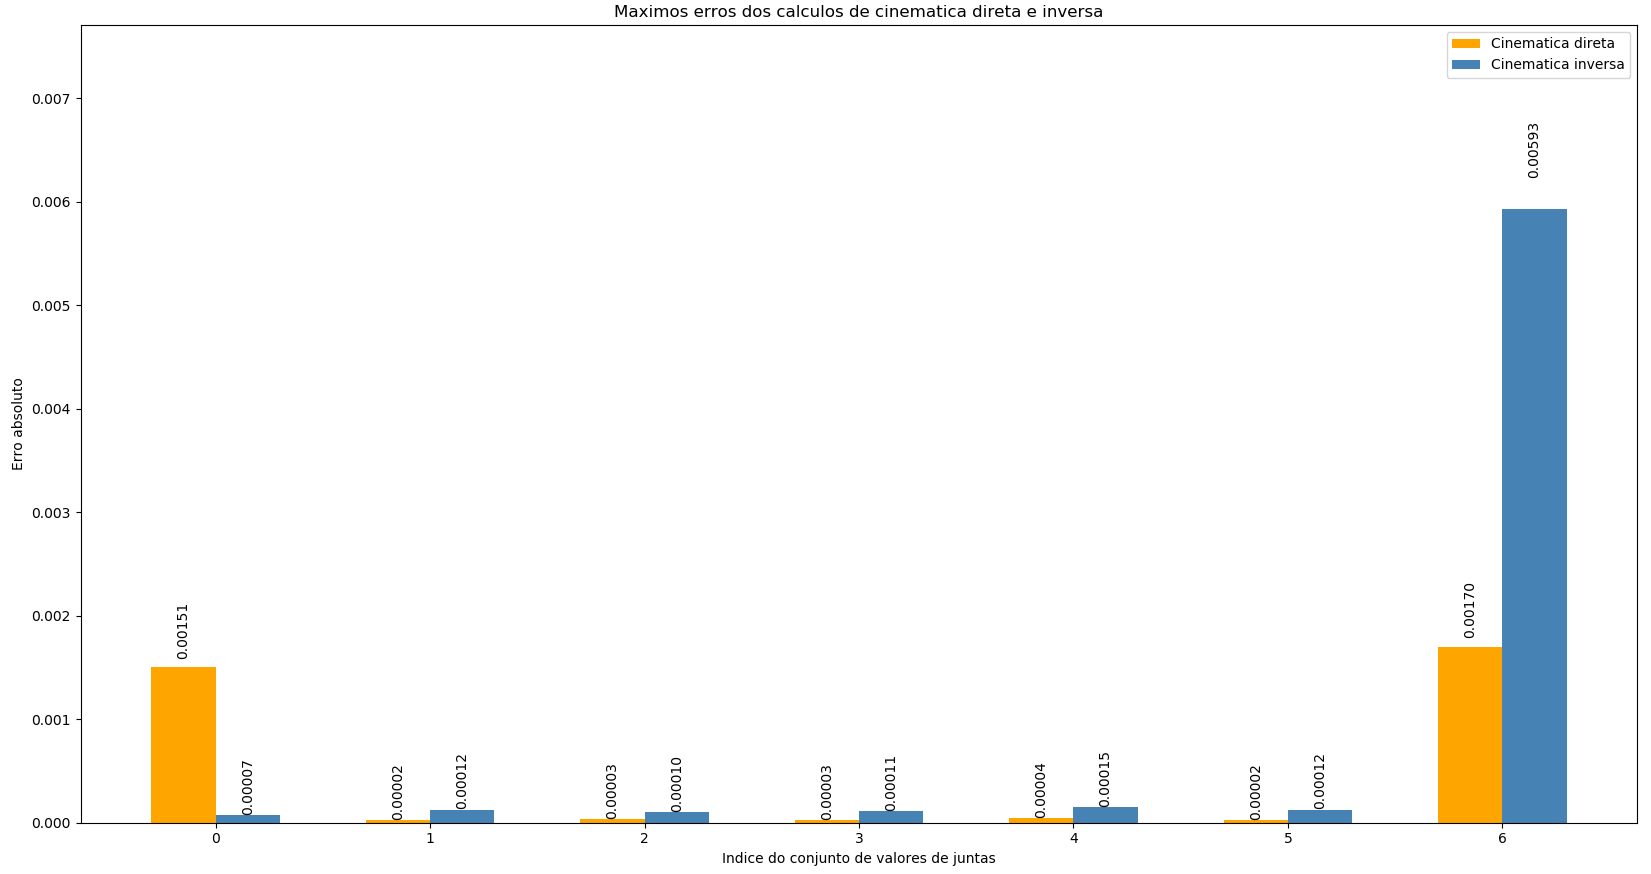
\includegraphics[width=\textwidth]{images/maximos_erros_set_2.png}
\end{figure}

\begin{figure}[htp]
	\centering
	\caption{Erros das 6 juntas do UR5 para cada conjunto da Tabela \ref{tab:conjuntos-de-valores-de-juntas-recortado}}
	\label{fig:grafico-erro-juntas-set-2}
	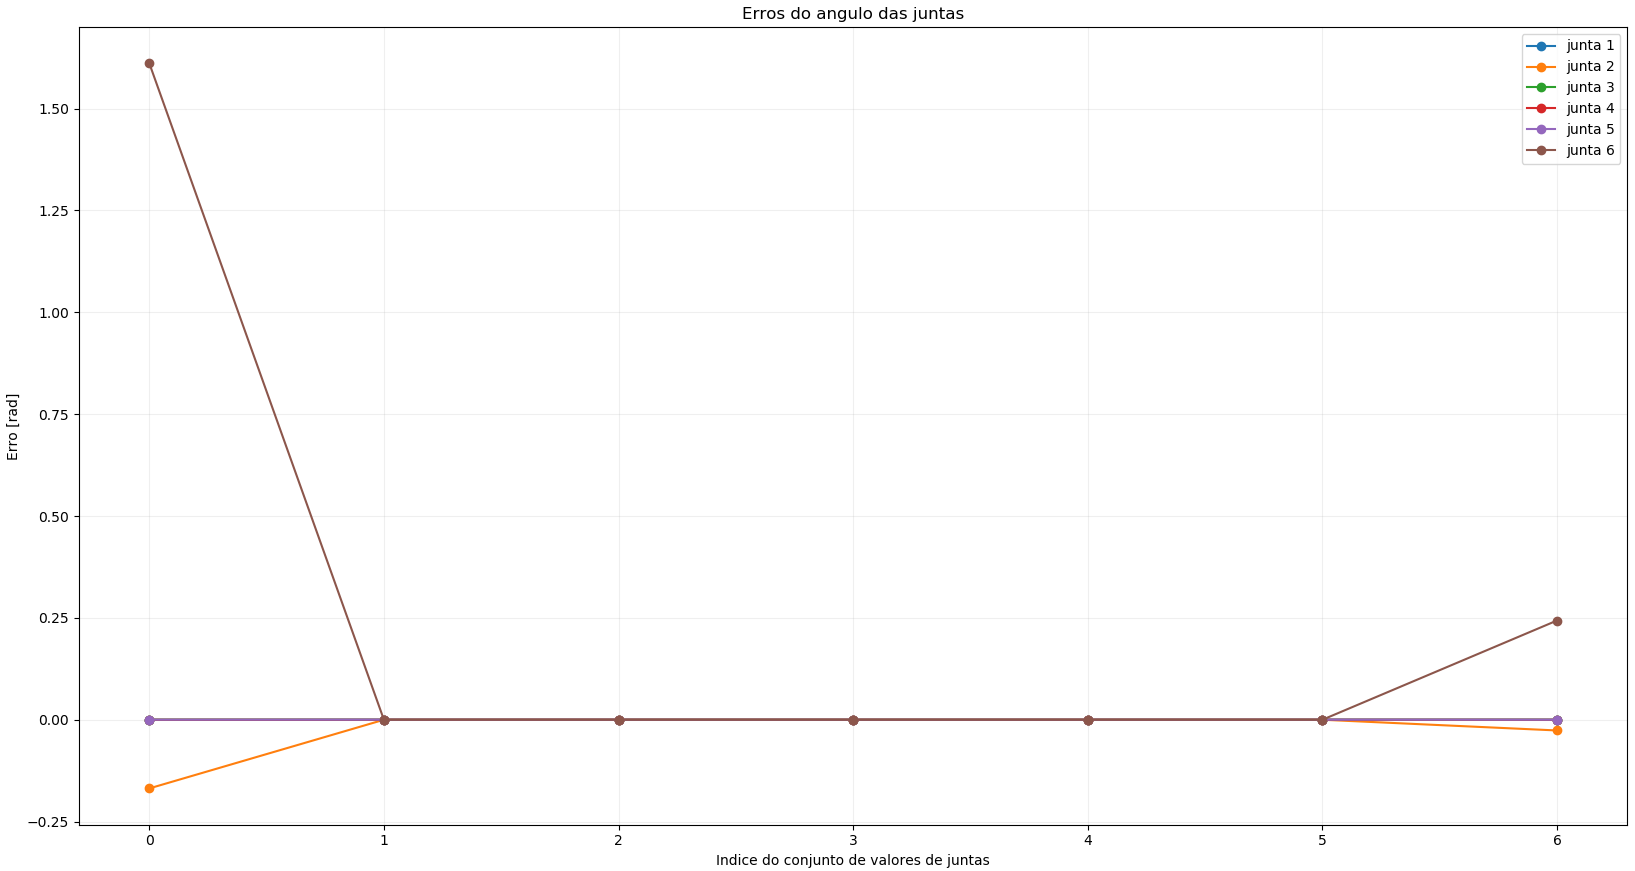
\includegraphics[width=\textwidth]{images/erro_do_angulo_das_juntas_set_2.png}
\end{figure}

\section{Planejamento de Trajetória}
O planjedor de trajetória tem a função de mapear a posição de cada junta 
durante o movimento. Esse componente deve ser utilizado afim de se suavizar o 
movimento dos motores para se evitar colisões e \textit{stress} desnecessário 
das juntas. Nesse trabalho, dois planejadores foram desenvolvidos e as trajetórias
planejadas e executadas foram comparadas. Os planejadores escolhidos foram o 
\textit{Linear Segment Parabolic Blend} (LSPB), o qual se gera uma trajetória trapezoidal
com velocidade e aceleração constantes, e o \textit{Cubic Polynomial} (polinomial),
 o qual se gera uma função polinomial cúbica de posição para ser seguida pelas juntas.

A implementação foi feita com base no livro do Mark Spong, de forma que ao se instanciar
o planejador, as curvas de posição, velocidade e aceleração são calculadas. Na imagem abaixo,
pode ser visto a comparação das trajetórias calculadas com o lspb em cima e o polinomial em baixo.
Se definiu a velocidade inicial e final do planejador polinomial como zero, visto que o LSPB já tem
essa restrição, então não seria uma comparação muito válida caso as condições iniciais e finais sejam
diferentes. Para o LSPB, se definiu uma velocidade arbitrária de -184 rad por segundo. Por fim, para 
ambos os planjadores, se determinou a posição inicial e final como 1.5 rad e -1.2 rad, e o tempo
inicial e final como 35.2 e 37.4 segundos. 

\begin{figure}[htp]
	\centering
	\caption{Planejamento de trajetória pelo método LSPB em cima e polinomial em baixo}
	\label{fig:comparacao-planejamento}
	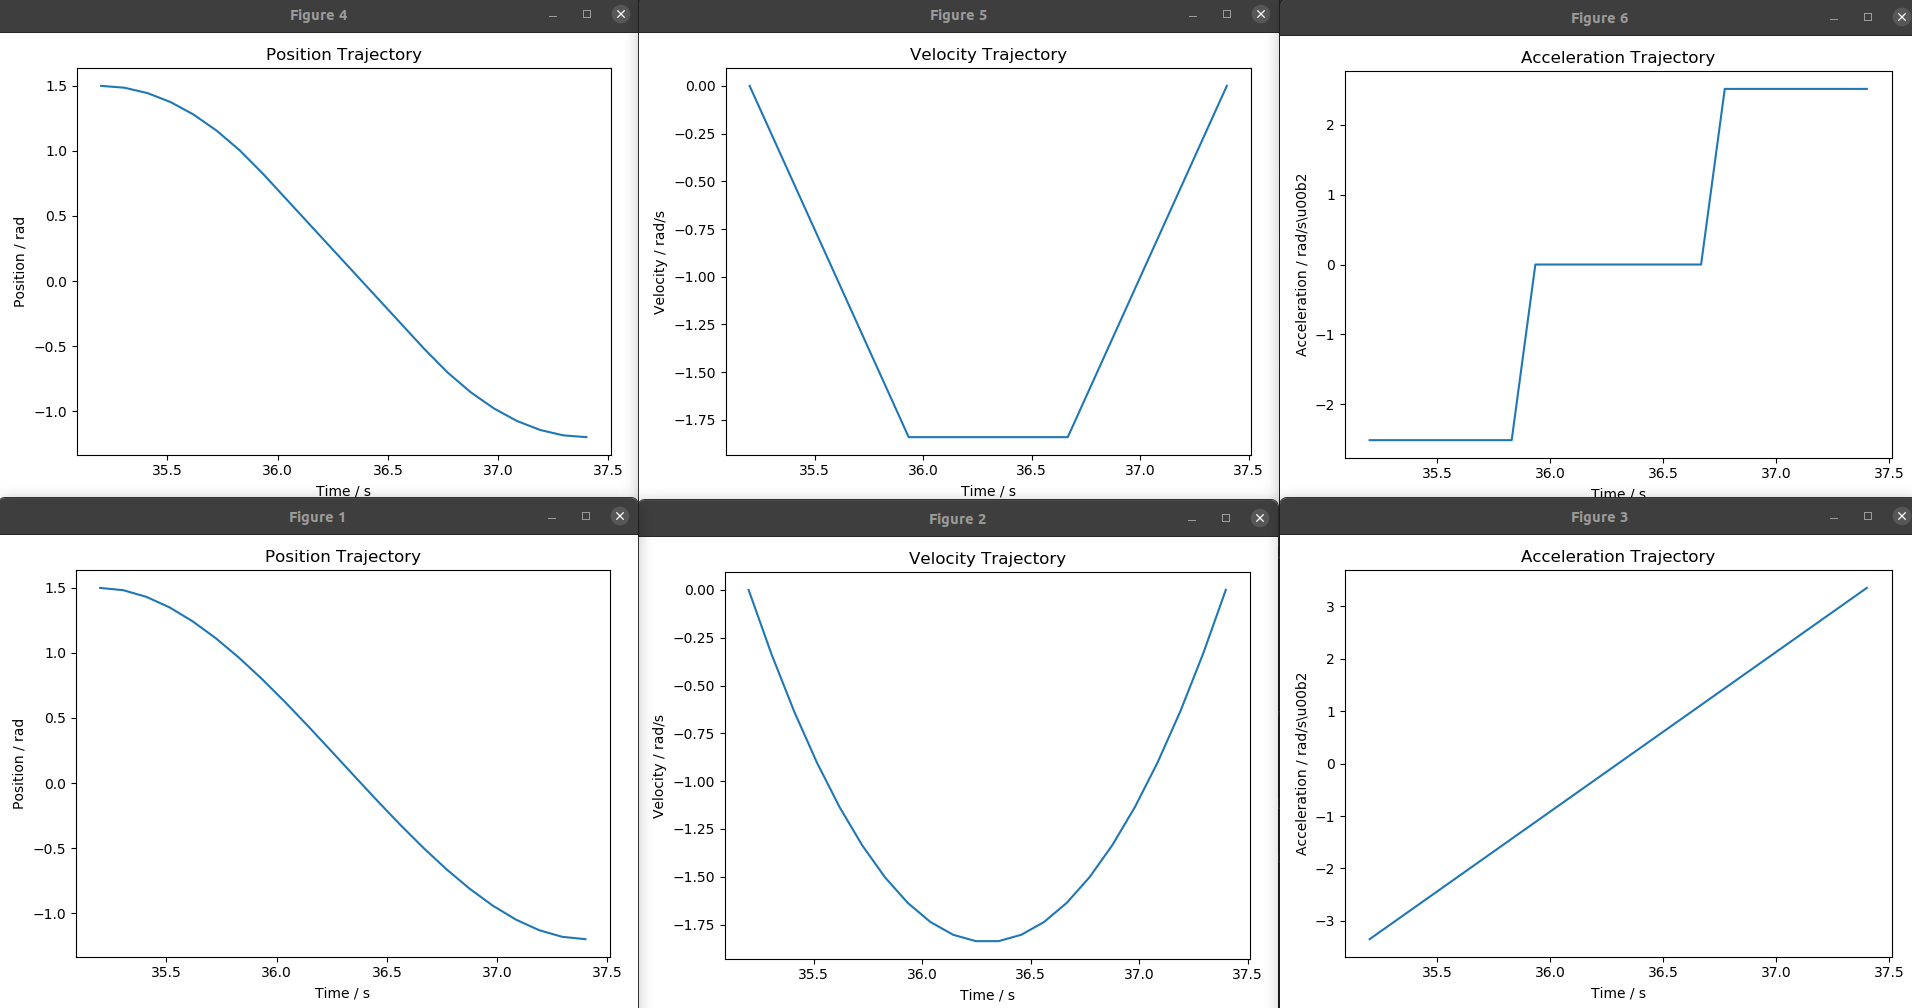
\includegraphics[width=\textwidth]{images/comparisson.png}
\end{figure}

Após a validação dos algoritmos de planjemento, estes foram testados em simulação para o deslocamento
do UR5. Abaixo, é possivel visualizar os gráficos do deslocamento de cada uma das 6 juntas utilizando
diferentes estratégias. A Figura\ref{fig:execucao-lspb} representa o movimento das juntas utilizando LSPB, 
Figura \ref{fig:execucao-polinomial} representa o movimento das juntas utilizando o planejamento polinomial, 
por fim, a Figura \ref{fig:execucao-pid} representa o movimento do braço sem nenhum planjedor, somente com 
o controle de posição das juntas.

\begin{figure}[htp]
	\centering
	\caption{Execução de trajetória pelo método LSPB}
	\label{fig:execucao-lspb}
	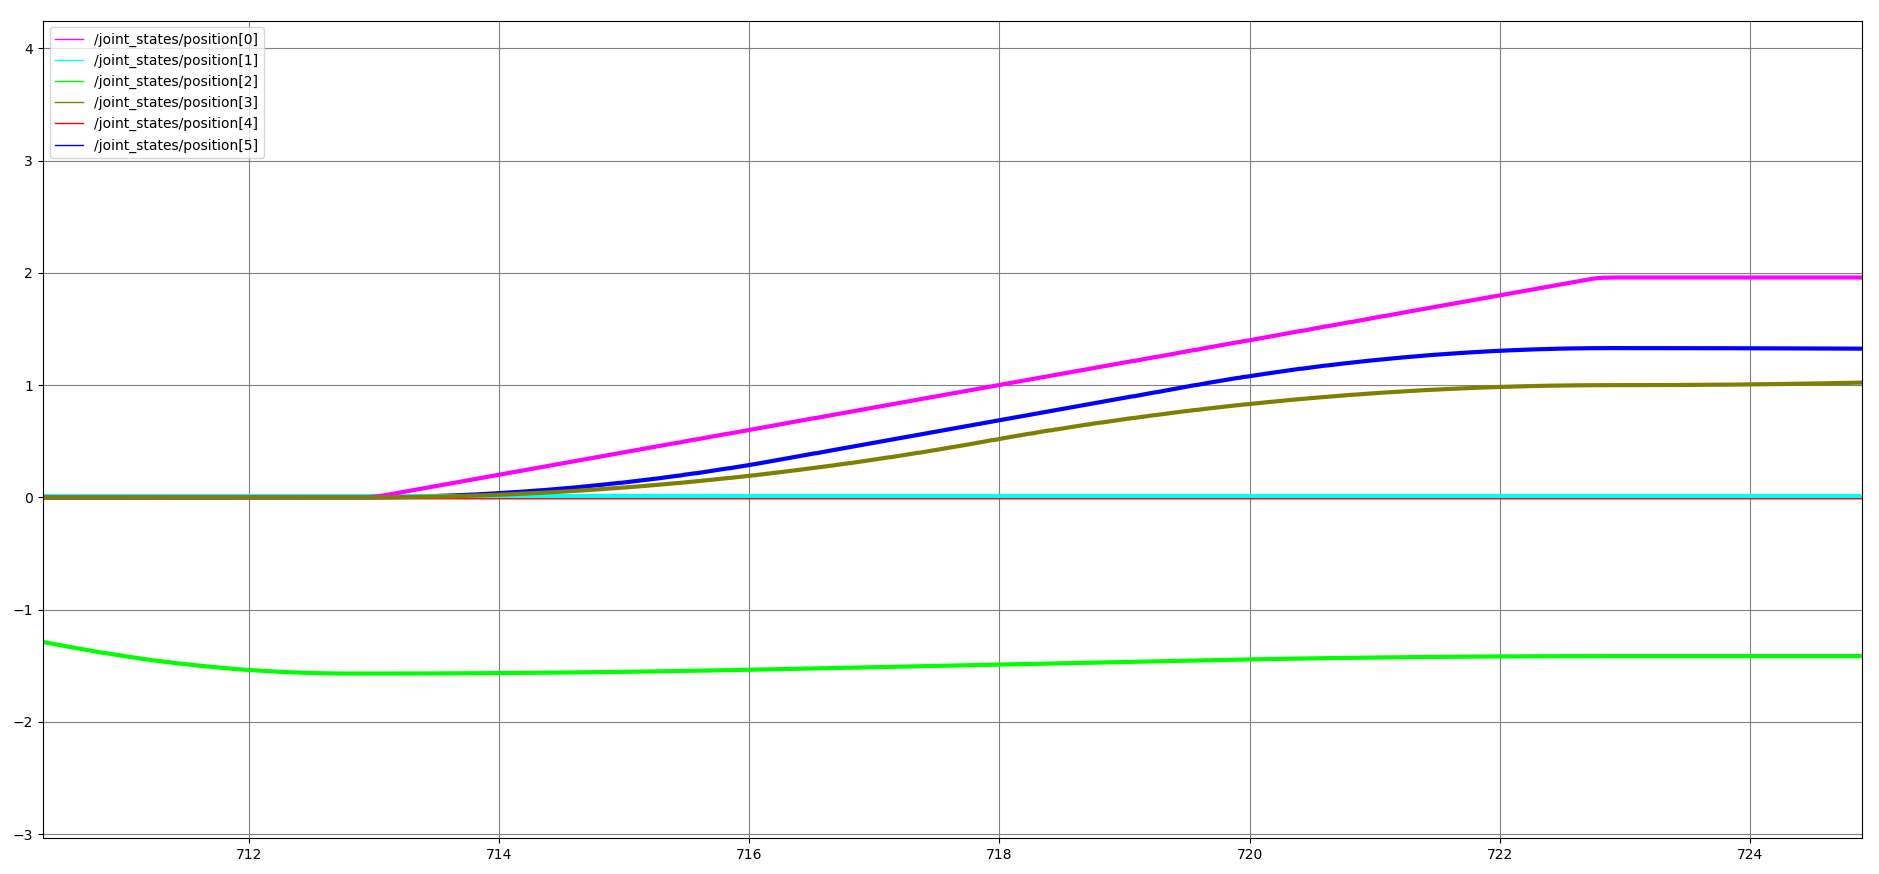
\includegraphics[width=\textwidth]{images/lspb.png}
\end{figure}

\begin{figure}[htp]
	\centering
	\caption{Execução de trajetória pelo método polinomial}
	\label{fig:execucao-polinomial}
	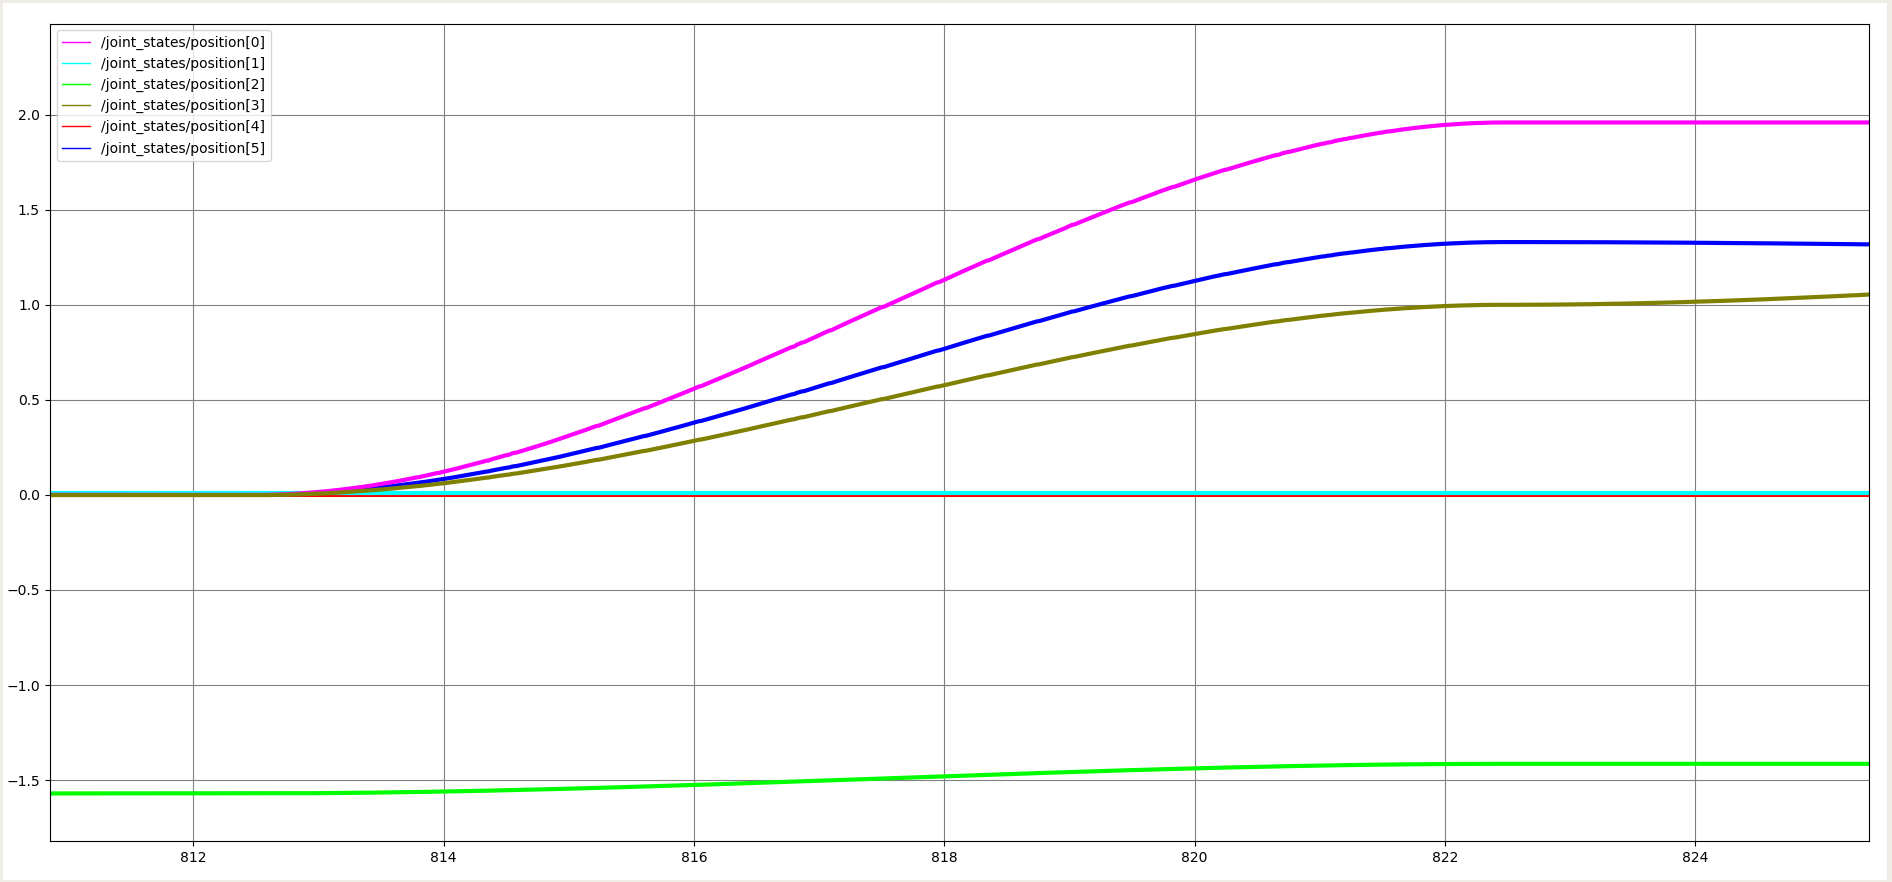
\includegraphics[width=\textwidth]{images/polinomial.png}
\end{figure}

\begin{figure}[htp]
	\centering
	\caption{Execução de trajetória sem planejamento}
	\label{fig:execucao-pid}
	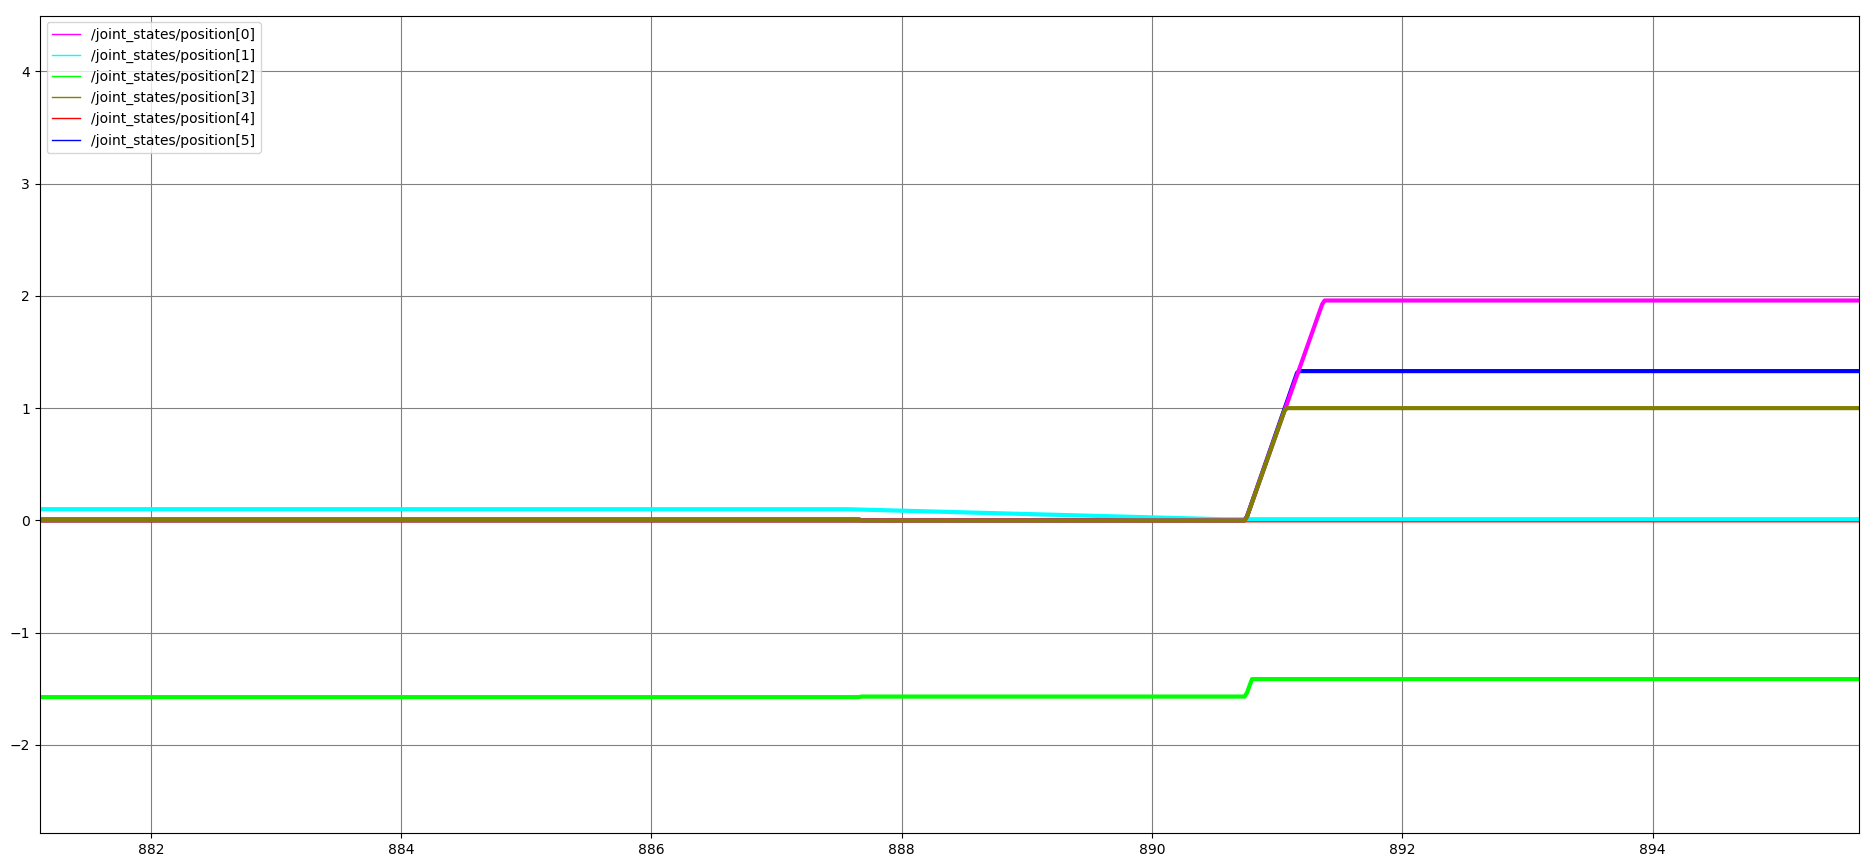
\includegraphics[width=\textwidth]{images/no_planner.png}
\end{figure}

Dessa forma, se conclue esse trabalho, no qual foi possível realizar a missão de 
se aproximar de uma lata, utilizando cinemática inversa e planejador de trajetórias 
próprios. 

\bibliographystyle{apalike}
\bibliography{references.bib}

\end{document}